% Options for packages loaded elsewhere
\PassOptionsToPackage{unicode}{hyperref}
\PassOptionsToPackage{hyphens}{url}
\PassOptionsToPackage{dvipsnames,svgnames,x11names}{xcolor}
%
\documentclass[
  letterpaper,
  DIV=11,
  numbers=noendperiod]{scrreprt}

\usepackage{amsmath,amssymb}
\usepackage{iftex}
\ifPDFTeX
  \usepackage[T1]{fontenc}
  \usepackage[utf8]{inputenc}
  \usepackage{textcomp} % provide euro and other symbols
\else % if luatex or xetex
  \usepackage{unicode-math}
  \defaultfontfeatures{Scale=MatchLowercase}
  \defaultfontfeatures[\rmfamily]{Ligatures=TeX,Scale=1}
\fi
\usepackage{lmodern}
\ifPDFTeX\else  
    % xetex/luatex font selection
\fi
% Use upquote if available, for straight quotes in verbatim environments
\IfFileExists{upquote.sty}{\usepackage{upquote}}{}
\IfFileExists{microtype.sty}{% use microtype if available
  \usepackage[]{microtype}
  \UseMicrotypeSet[protrusion]{basicmath} % disable protrusion for tt fonts
}{}
\makeatletter
\@ifundefined{KOMAClassName}{% if non-KOMA class
  \IfFileExists{parskip.sty}{%
    \usepackage{parskip}
  }{% else
    \setlength{\parindent}{0pt}
    \setlength{\parskip}{6pt plus 2pt minus 1pt}}
}{% if KOMA class
  \KOMAoptions{parskip=half}}
\makeatother
\usepackage{xcolor}
\setlength{\emergencystretch}{3em} % prevent overfull lines
\setcounter{secnumdepth}{5}
% Make \paragraph and \subparagraph free-standing
\makeatletter
\ifx\paragraph\undefined\else
  \let\oldparagraph\paragraph
  \renewcommand{\paragraph}{
    \@ifstar
      \xxxParagraphStar
      \xxxParagraphNoStar
  }
  \newcommand{\xxxParagraphStar}[1]{\oldparagraph*{#1}\mbox{}}
  \newcommand{\xxxParagraphNoStar}[1]{\oldparagraph{#1}\mbox{}}
\fi
\ifx\subparagraph\undefined\else
  \let\oldsubparagraph\subparagraph
  \renewcommand{\subparagraph}{
    \@ifstar
      \xxxSubParagraphStar
      \xxxSubParagraphNoStar
  }
  \newcommand{\xxxSubParagraphStar}[1]{\oldsubparagraph*{#1}\mbox{}}
  \newcommand{\xxxSubParagraphNoStar}[1]{\oldsubparagraph{#1}\mbox{}}
\fi
\makeatother

\usepackage{color}
\usepackage{fancyvrb}
\newcommand{\VerbBar}{|}
\newcommand{\VERB}{\Verb[commandchars=\\\{\}]}
\DefineVerbatimEnvironment{Highlighting}{Verbatim}{commandchars=\\\{\}}
% Add ',fontsize=\small' for more characters per line
\usepackage{framed}
\definecolor{shadecolor}{RGB}{241,243,245}
\newenvironment{Shaded}{\begin{snugshade}}{\end{snugshade}}
\newcommand{\AlertTok}[1]{\textcolor[rgb]{0.68,0.00,0.00}{#1}}
\newcommand{\AnnotationTok}[1]{\textcolor[rgb]{0.37,0.37,0.37}{#1}}
\newcommand{\AttributeTok}[1]{\textcolor[rgb]{0.40,0.45,0.13}{#1}}
\newcommand{\BaseNTok}[1]{\textcolor[rgb]{0.68,0.00,0.00}{#1}}
\newcommand{\BuiltInTok}[1]{\textcolor[rgb]{0.00,0.23,0.31}{#1}}
\newcommand{\CharTok}[1]{\textcolor[rgb]{0.13,0.47,0.30}{#1}}
\newcommand{\CommentTok}[1]{\textcolor[rgb]{0.37,0.37,0.37}{#1}}
\newcommand{\CommentVarTok}[1]{\textcolor[rgb]{0.37,0.37,0.37}{\textit{#1}}}
\newcommand{\ConstantTok}[1]{\textcolor[rgb]{0.56,0.35,0.01}{#1}}
\newcommand{\ControlFlowTok}[1]{\textcolor[rgb]{0.00,0.23,0.31}{\textbf{#1}}}
\newcommand{\DataTypeTok}[1]{\textcolor[rgb]{0.68,0.00,0.00}{#1}}
\newcommand{\DecValTok}[1]{\textcolor[rgb]{0.68,0.00,0.00}{#1}}
\newcommand{\DocumentationTok}[1]{\textcolor[rgb]{0.37,0.37,0.37}{\textit{#1}}}
\newcommand{\ErrorTok}[1]{\textcolor[rgb]{0.68,0.00,0.00}{#1}}
\newcommand{\ExtensionTok}[1]{\textcolor[rgb]{0.00,0.23,0.31}{#1}}
\newcommand{\FloatTok}[1]{\textcolor[rgb]{0.68,0.00,0.00}{#1}}
\newcommand{\FunctionTok}[1]{\textcolor[rgb]{0.28,0.35,0.67}{#1}}
\newcommand{\ImportTok}[1]{\textcolor[rgb]{0.00,0.46,0.62}{#1}}
\newcommand{\InformationTok}[1]{\textcolor[rgb]{0.37,0.37,0.37}{#1}}
\newcommand{\KeywordTok}[1]{\textcolor[rgb]{0.00,0.23,0.31}{\textbf{#1}}}
\newcommand{\NormalTok}[1]{\textcolor[rgb]{0.00,0.23,0.31}{#1}}
\newcommand{\OperatorTok}[1]{\textcolor[rgb]{0.37,0.37,0.37}{#1}}
\newcommand{\OtherTok}[1]{\textcolor[rgb]{0.00,0.23,0.31}{#1}}
\newcommand{\PreprocessorTok}[1]{\textcolor[rgb]{0.68,0.00,0.00}{#1}}
\newcommand{\RegionMarkerTok}[1]{\textcolor[rgb]{0.00,0.23,0.31}{#1}}
\newcommand{\SpecialCharTok}[1]{\textcolor[rgb]{0.37,0.37,0.37}{#1}}
\newcommand{\SpecialStringTok}[1]{\textcolor[rgb]{0.13,0.47,0.30}{#1}}
\newcommand{\StringTok}[1]{\textcolor[rgb]{0.13,0.47,0.30}{#1}}
\newcommand{\VariableTok}[1]{\textcolor[rgb]{0.07,0.07,0.07}{#1}}
\newcommand{\VerbatimStringTok}[1]{\textcolor[rgb]{0.13,0.47,0.30}{#1}}
\newcommand{\WarningTok}[1]{\textcolor[rgb]{0.37,0.37,0.37}{\textit{#1}}}

\providecommand{\tightlist}{%
  \setlength{\itemsep}{0pt}\setlength{\parskip}{0pt}}\usepackage{longtable,booktabs,array}
\usepackage{calc} % for calculating minipage widths
% Correct order of tables after \paragraph or \subparagraph
\usepackage{etoolbox}
\makeatletter
\patchcmd\longtable{\par}{\if@noskipsec\mbox{}\fi\par}{}{}
\makeatother
% Allow footnotes in longtable head/foot
\IfFileExists{footnotehyper.sty}{\usepackage{footnotehyper}}{\usepackage{footnote}}
\makesavenoteenv{longtable}
\usepackage{graphicx}
\makeatletter
\newsavebox\pandoc@box
\newcommand*\pandocbounded[1]{% scales image to fit in text height/width
  \sbox\pandoc@box{#1}%
  \Gscale@div\@tempa{\textheight}{\dimexpr\ht\pandoc@box+\dp\pandoc@box\relax}%
  \Gscale@div\@tempb{\linewidth}{\wd\pandoc@box}%
  \ifdim\@tempb\p@<\@tempa\p@\let\@tempa\@tempb\fi% select the smaller of both
  \ifdim\@tempa\p@<\p@\scalebox{\@tempa}{\usebox\pandoc@box}%
  \else\usebox{\pandoc@box}%
  \fi%
}
% Set default figure placement to htbp
\def\fps@figure{htbp}
\makeatother
% definitions for citeproc citations
\NewDocumentCommand\citeproctext{}{}
\NewDocumentCommand\citeproc{mm}{%
  \begingroup\def\citeproctext{#2}\cite{#1}\endgroup}
\makeatletter
 % allow citations to break across lines
 \let\@cite@ofmt\@firstofone
 % avoid brackets around text for \cite:
 \def\@biblabel#1{}
 \def\@cite#1#2{{#1\if@tempswa , #2\fi}}
\makeatother
\newlength{\cslhangindent}
\setlength{\cslhangindent}{1.5em}
\newlength{\csllabelwidth}
\setlength{\csllabelwidth}{3em}
\newenvironment{CSLReferences}[2] % #1 hanging-indent, #2 entry-spacing
 {\begin{list}{}{%
  \setlength{\itemindent}{0pt}
  \setlength{\leftmargin}{0pt}
  \setlength{\parsep}{0pt}
  % turn on hanging indent if param 1 is 1
  \ifodd #1
   \setlength{\leftmargin}{\cslhangindent}
   \setlength{\itemindent}{-1\cslhangindent}
  \fi
  % set entry spacing
  \setlength{\itemsep}{#2\baselineskip}}}
 {\end{list}}
\usepackage{calc}
\newcommand{\CSLBlock}[1]{\hfill\break\parbox[t]{\linewidth}{\strut\ignorespaces#1\strut}}
\newcommand{\CSLLeftMargin}[1]{\parbox[t]{\csllabelwidth}{\strut#1\strut}}
\newcommand{\CSLRightInline}[1]{\parbox[t]{\linewidth - \csllabelwidth}{\strut#1\strut}}
\newcommand{\CSLIndent}[1]{\hspace{\cslhangindent}#1}

<style>
h1.unlisted {
  display: none;
}
</style>
\KOMAoption{captions}{tableheading}
\makeatletter
\@ifpackageloaded{tcolorbox}{}{\usepackage[skins,breakable]{tcolorbox}}
\@ifpackageloaded{fontawesome5}{}{\usepackage{fontawesome5}}
\definecolor{quarto-callout-color}{HTML}{909090}
\definecolor{quarto-callout-note-color}{HTML}{0758E5}
\definecolor{quarto-callout-important-color}{HTML}{CC1914}
\definecolor{quarto-callout-warning-color}{HTML}{EB9113}
\definecolor{quarto-callout-tip-color}{HTML}{00A047}
\definecolor{quarto-callout-caution-color}{HTML}{FC5300}
\definecolor{quarto-callout-color-frame}{HTML}{acacac}
\definecolor{quarto-callout-note-color-frame}{HTML}{4582ec}
\definecolor{quarto-callout-important-color-frame}{HTML}{d9534f}
\definecolor{quarto-callout-warning-color-frame}{HTML}{f0ad4e}
\definecolor{quarto-callout-tip-color-frame}{HTML}{02b875}
\definecolor{quarto-callout-caution-color-frame}{HTML}{fd7e14}
\makeatother
\makeatletter
\@ifpackageloaded{bookmark}{}{\usepackage{bookmark}}
\makeatother
\makeatletter
\@ifpackageloaded{caption}{}{\usepackage{caption}}
\AtBeginDocument{%
\ifdefined\contentsname
  \renewcommand*\contentsname{Table of contents}
\else
  \newcommand\contentsname{Table of contents}
\fi
\ifdefined\listfigurename
  \renewcommand*\listfigurename{List of Figures}
\else
  \newcommand\listfigurename{List of Figures}
\fi
\ifdefined\listtablename
  \renewcommand*\listtablename{List of Tables}
\else
  \newcommand\listtablename{List of Tables}
\fi
\ifdefined\figurename
  \renewcommand*\figurename{Figure}
\else
  \newcommand\figurename{Figure}
\fi
\ifdefined\tablename
  \renewcommand*\tablename{Table}
\else
  \newcommand\tablename{Table}
\fi
}
\@ifpackageloaded{float}{}{\usepackage{float}}
\floatstyle{ruled}
\@ifundefined{c@chapter}{\newfloat{codelisting}{h}{lop}}{\newfloat{codelisting}{h}{lop}[chapter]}
\floatname{codelisting}{Listing}
\newcommand*\listoflistings{\listof{codelisting}{List of Listings}}
\makeatother
\makeatletter
\makeatother
\makeatletter
\@ifpackageloaded{caption}{}{\usepackage{caption}}
\@ifpackageloaded{subcaption}{}{\usepackage{subcaption}}
\makeatother
\newcounter{quartocalloutcauno}
\newcommand{\quartocalloutcau}[1]{\refstepcounter{quartocalloutcauno}\label{#1}}
\newcounter{quartocallouttipno}
\newcommand{\quartocallouttip}[1]{\refstepcounter{quartocallouttipno}\label{#1}}

\usepackage{bookmark}

\IfFileExists{xurl.sty}{\usepackage{xurl}}{} % add URL line breaks if available
\urlstyle{same} % disable monospaced font for URLs
\hypersetup{
  pdftitle={evoland+ HPC},
  pdfauthor={Carlson Büth and Benjamin Black},
  colorlinks=true,
  linkcolor={blue},
  filecolor={Maroon},
  citecolor={Blue},
  urlcolor={Blue},
  pdfcreator={LaTeX via pandoc}}


\title{evoland+ HPC}
\author{Carlson Büth and Benjamin Black}
\date{Invalid Date}

\begin{document}
\maketitle

\renewcommand*\contentsname{Table of contents}
{
\hypersetup{linkcolor=}
\setcounter{tocdepth}{2}
\tableofcontents
}

\bookmarksetup{startatroot}

\chapter*{evoland+ HPC Guide}\label{evoland-hpc-guide}

\markboth{evoland+ HPC Guide}{evoland+ HPC Guide}

\phantomsection\label{about}

\newpage{}

\subsection*{An unified pipeline for scenario based modelling of Land
Use and Land Cover Change, Ecosystem Services and
(?)}\label{an-unified-pipeline-for-scenario-based-modelling-of-land-use-and-land-cover-change-ecosystem-services-and}
\addcontentsline{toc}{subsection}{An unified pipeline for scenario based
modelling of Land Use and Land Cover Change, Ecosystem Services and (?)}

\begin{itemize}
\tightlist
\item
  \href{https://github.com/blenback/LULCC-CH}{Land use land cover change
  (LULCC) model for Switzerland} (Black et al. 2023; Black et al. 2024)
\item
  \href{https://github.com/N-SDM/N-SDM}{Species distribution modelling
  (N-SDM)} (Adde et al. 2023)
\item
  Nature's contributions to people (NCP) calculations, based on (Külling
  et al. 2024)
\end{itemize}

\bookmarksetup{startatroot}

\chapter*{\texorpdfstring{What is
\emph{Future-EI}?}{What is Future-EI?}}\label{what-is-future-ei}
\addcontentsline{toc}{chapter}{What is \emph{Future-EI}?}

\markboth{What is \emph{Future-EI}?}{What is \emph{Future-EI}?}

This is a guide and reference book for the Future-EI pipeline. To
explore future ecosystem services and nature's contributions to people
(NCP) in the context of climate scenarios, Future-EI (future ecological
infrastructure) couples the , , and NCP calculations .

For more details on the background on the Future-EI pipeline, see the
\href{intro.qmd}{Introduction}.

Open Source, High Performance Computing, Reproducibility

\ldots{}

\section*{Statement of need}\label{statement-of-need}
\addcontentsline{toc}{section}{Statement of need}

\markright{Statement of need}

\emph{illustrate the research purpose of the software and place it in
the context of related work}

\section*{Acknowledgements}\label{acknowledgements}
\addcontentsline{toc}{section}{Acknowledgements}

\markright{Acknowledgements}

This project was funded under the
\href{https://valpar.ch/index_en.php?page=home_en}{ValPar.CH} project,
funded as part of a pilot project of the ``Action Plan for the Swiss
Biodiversity Strategy (AP SBS)'' by the Federal Office for the
Environment (FOEN).

\href{https://github.com/N-SDM/N-SDM}{N-SDM} has been developed within
the \href{https://www.unil.ch/ecospat/en/home.html}{Ecospatial Ecology
Group (Ecospat)} at the
\href{https://www.unil.ch/central/en/home.html}{University of Lausanne}

\href{https://github.com/blenback/LULCC-CH}{LULCC-CH}\ldots{}

\section*{How to cite}\label{how-to-cite}
\addcontentsline{toc}{section}{How to cite}

\markright{How to cite}

When using the Future-EI pipeline, please cite the following paper:

\begin{Shaded}
\begin{Highlighting}[]
\CommentTok{\# also update in paper.bib when published}
\VariableTok{@unpublished}\NormalTok{\{}\OtherTok{Black2025}\NormalTok{,}
  \DataTypeTok{title}\NormalTok{=\{Future{-}EI Paper\},}
  \DataTypeTok{author}\NormalTok{=\{Black, Ben and others\},}
\NormalTok{\}}
\end{Highlighting}
\end{Shaded}

\section*{Get started with Future-EI}\label{get-started-with-future-ei}
\addcontentsline{toc}{section}{Get started with Future-EI}

\markright{Get started with Future-EI}

\href{intro.qmd}{Introduction}

\href{structure.qmd}{Structure}

\href{pipeline/setup.qmd}{Setup}

\bookmarksetup{startatroot}

\chapter{Introduction}\label{introduction}

Details on the background on the evoland+ HPC pipeline

\begin{itemize}
\tightlist
\item
  Motivation
\item
  Why
\item
  Climate Scenarios

  \begin{itemize}
  \tightlist
  \item
    many → high computational demand
  \end{itemize}
\item
  Cite Mayer, Rabe, and Grêt-Regamey (2023), Black et al. (2023), Adde
  et al. (2023)
\item
  Related work
\end{itemize}

Structure of the next sections:

\begin{itemize}
\tightlist
\item
  The \hyperref[introduction]{Introduction} you read
\item
  \href{structure.html}{Structure} gives an overview of the pipeline
\item
  \href{pipeline/}{Pipeline} describes the setup and steps in detail
\item
  \href{summary.html}{Summary} concludes the guide
\item
  \href{references.html}{References} list all cited works
\end{itemize}

\bookmarksetup{startatroot}

\chapter{Structure}\label{structure}

For the related research project Black et al. (n.d.), we couple three
main steps: Land Use Simulation, combined NCP Estimations and Species
Distribution Modeling. These are shown bold in the
Figure~\ref{fig-pipeline}. Future-EI covers the LULC Simulation and
steps dependent on its output, namely the NCP estimations, intensity
analysis and focal window preparation. These steps, shown in blue, are
unified to be automated for command line interface (CLI) and high
performance computing (HPC) compatibility, to be scalable and
reproducible.

\begin{figure}

\centering{

\includegraphics[width=5.28in,height=6.06in]{structure_files/figure-latex/mermaid-figure-1.png}

}

\caption{\label{fig-pipeline}Pipeline Overview -- Steps in blue are part
of the Future-EI pipeline, red steps are external. From this structure,
a clear order of execution can be derived.}

\end{figure}%

First, we give an overview of each step in the pipeline. In contrast,
the \hyperref[pipeline]{Pipeline} section details and documents the
individual steps and code used, in terms of input, output and execution.

\section{LULCC: Land Use Simulation}\label{lulcc-land-use-simulation}

The \href{https://github.com/blenback/LULCC-CH}{land use land cover
change (LULCC) model for Switzerland} (Black et al. 2023; Black et al.
2024) is the first step in the Future-EI pipeline. For given climate
scenarios, it simulates land use changes in Switzerland until a given
future year (e.g., 2060), based on historical data and future
projections. The generated land use maps are then used as input for the
following steps.

\section{NCP: Nature's Contributions to
People}\label{ncp-natures-contributions-to-people}

A range of NCP are estimated from the land use maps. Some NCP use
further data for the estimation, e.g., precipitation and temperature
projections.

The code is based on Külling et al. (2024), but has been adapted for
automation and HPC compatibility.

\begin{longtable}[]{@{}
  >{\raggedleft\arraybackslash}p{(\linewidth - 4\tabcolsep) * \real{0.1092}}
  >{\raggedright\arraybackslash}p{(\linewidth - 4\tabcolsep) * \real{0.4706}}
  >{\raggedright\arraybackslash}p{(\linewidth - 4\tabcolsep) * \real{0.4202}}@{}}
\caption{Nature's Contributions to People (NCP) estimated from the LULCC
model. }\label{tbl-ncp}\tabularnewline
\toprule\noalign{}
\begin{minipage}[b]{\linewidth}\raggedleft
NCP
\end{minipage} & \begin{minipage}[b]{\linewidth}\raggedright
Name
\end{minipage} & \begin{minipage}[b]{\linewidth}\raggedright
Indicator
\end{minipage} \\
\midrule\noalign{}
\endfirsthead
\toprule\noalign{}
\begin{minipage}[b]{\linewidth}\raggedleft
NCP
\end{minipage} & \begin{minipage}[b]{\linewidth}\raggedright
Name
\end{minipage} & \begin{minipage}[b]{\linewidth}\raggedright
Indicator
\end{minipage} \\
\midrule\noalign{}
\endhead
\bottomrule\noalign{}
\endlastfoot
\hyperref[CAR]{CAR} & Regulation of climate & Carbon stored in biomass
and soil \\
\hyperref[FF]{FF} & Food and feed & Crop production potential
(\texttt{ecocrop}) \\
\hyperref[HAB]{HAB} & Habitat creation and maintenance & Habitat quality
index \\
\hyperref[NDR]{NDR} & Nutrient Delivery Ratio & Annual nutrient
retention by vegetation \\
\hyperref[POL]{POL} & Pollination and dispersal of seeds & Habitat
abundance for pollinators \\
\hyperref[REC]{REC} & Recreation potential & Recreation potential (RP)
provided by ecosystems \\
\hyperref[SDR]{SDR} & Formation, protection and decontamination of soils
& Erosion control by sediment retention \\
\hyperref[WY]{WY} & Regulation of freshwater quantity, location and
timing & Annual water yield \\
\end{longtable}

\section{Intensity Analysis}\label{intensity-analysis}

The Intensity Analysis (IA) is based on x, and serves as

\section{Focal LULC Preparation}\label{focal-lulc-preparation}

\emph{Explain why} These focal layers are used as inputs for X and Y,
and act as NCP, specifically Z.

\section{N-SDM: Nested Species Distribution
Modelling}\label{n-sdm-nested-species-distribution-modelling}

The \href{https://github.com/N-SDM/N-SDM}{nested species distribution
modelling (N-SDM)} (Adde et al. 2023) step simulates the distribution of
species in Switzerland. Species occurrence used to fit models and
covariate data are selected, both at different spatial scales, to
predict the species distribution. This part is not integrated into the
Future-EI pipeline, and needs to be consulted separately.

\section{Species Maps Aggregation}\label{species-maps-aggregation}

The species maps are then aggregated to \ldots{}

\section{Clustering}\label{clustering}

To analyze the scenarios, the species maps are clustered to \ldots{} The
code for this step can be found in the separate repository
\href{https://github.com/blenback/reponame}{reponame}. These scripts are
adapted to the case of Switzerland and the Future-EI project. \ldots{}

\bookmarksetup{startatroot}

\chapter{Pipeline}\label{pipeline}

The Future-EI pipeline consists out of various scripts that can be found
in the \texttt{src} directory. For each included step of
Figure~\ref{fig-pipeline}, there is a subdirectory in
\texttt{src/steps}.

This part is structured as follows:

\begin{itemize}
\tightlist
\item
  \href{setup.html}{Setup}
\item
  Steps

  \begin{itemize}
  \tightlist
  \item
    \href{10_LULCC.html}{LULCC}
  \item
    \href{11_CheckLULCC.html}{Check LULCC}
  \item
    \href{20_FocalLULC.html}{Focals}
  \item
    \href{40_NCPs.html}{NCP}
  \end{itemize}
\item
  \href{running.html}{Running the pipeline}
\end{itemize}

The task of the Future-EI pipeline is to streamline the process, so that
varying the climate scenarios and other parameters can be carried out
efficiently. Introducing parallelization through
\href{https://slurm.schedmd.com/overview.html}{SLURM} batch jobs, and
adding HPC compatibility, are the main tasks of the pipeline. Meanwhile,
the pipeline keeps track of the intermediate results, a centralized
configuration file, and the execution of each step. Details on the
individual steps are given in the following sections.

\bookmarksetup{startatroot}

\chapter{Setup}\label{setup}

Before you set up the Future-EI pipeline, you should make sure to
satisfy a few requirements. This section will go over
\hyperref[hardware]{hardware} and \hyperref[software]{software}
requirements, and then guide you through the
\hyperref[future-ei-repository]{Future-EI repository} setup. The
following pages guide through the details of each step in the pipeline,
before concluding with the \href{running.html}{execution} of the
pipeline.

\subsection{Requirements}\label{requirements}

We are using a Linux cluster with
\href{https://slurm.schedmd.com/overview.html}{SLURM} as scheduler. If
your cluster uses a different scheduler, you can see if it is compatible
with the SLURM syntax, or you can adapt the scripts to your scheduler.

\begin{tcolorbox}[enhanced jigsaw, breakable, bottomrule=.15mm, toprule=.15mm, rightrule=.15mm, opacitybacktitle=0.6, title=\textcolor{quarto-callout-note-color}{\faInfo}\hspace{0.5em}{Note \ref*{cau-linux-cluster}: What is a Linux cluster?}, coltitle=black, colback=white, titlerule=0mm, toptitle=1mm, left=2mm, bottomtitle=1mm, colbacktitle=quarto-callout-note-color!10!white, colframe=quarto-callout-note-color-frame, opacityback=0, leftrule=.75mm, arc=.35mm]

\quartocalloutcau{cau-linux-cluster} 

As this pipeline is specifically designed to simulate a large number of
scenarios, it has been optimized for high-performance computing (HPC)
environments. If you only need to run a few scenarios, it might be
easier to run the steps manually. Otherwise, you do need to have access
to a Linux cluster with SLURM. Feel free to reach out to a technically
savvy colleague or your local HPC support for help.

\end{tcolorbox}

\subsubsection{Hardware}\label{hardware}

The minimum memory and CPU requirements cannot generally be stated, as
they depend on the area of interest, input data, and the number of
scenarios. A viable starting point for a country with the size of
Switzerland, using a resolution of 100~m, is 16~GB of memory and 4~CPUs.
This is the case for a few scenarios and no parallelization within the
steps. Scaling up to around 1000 scenarios, we suggest at least 128~GB
of memory and 16~CPUs, to achieve a viable runtime. As this is an
estimate, it is essential to monitor runtime before scaling up.

\subsubsection{Software}\label{software}

Additionally, you need to install the following software:

\paragraph{Micromamba/Conda}\label{micromambaconda}

For some pipeline steps, we use conda environments.
\href{https://docs.conda.io/projects/conda/en/stable/}{Conda} is a
package manager that helps you manage dependencies in isolated
environments. We recommend using
\href{https://mamba.readthedocs.io/en/latest/}{\texttt{micromamba}},
which does the same job as Conda, but resolves dependencies much faster,
with the flexibility of
\href{https://docs.conda.io/en/latest/miniconda.html}{\texttt{miniconda}}
(CLI of Conda). Find the installation instructions for Micromamba
\href{https://mamba.readthedocs.io/en/latest/installation/micromamba-installation.html}{here}.
We have added compatibility for \texttt{micromamba}, \texttt{mamba} and
\texttt{conda}, in this order of preference, but only tested with
\texttt{micromamba}\footnote{The installed CLI is identified via bash
  variables in
  \href{https://github.com/cbueth/Future-EI/tree/main/src/bash_common.sh}{\texttt{src/bash\_common.sh}}.
  If none is found, an error highlights the issue.}.

We have chosen \href{https://conda-forge.org/}{\texttt{conda-forge}} as
the default channel for the conda environments, as it is a single source
for our \texttt{R}, Python, and lower-level dependencies (e.g.,
\texttt{gdal}, \texttt{proj}). This is independent of the modules and
applications provided by the HPC environment.

\paragraph{Apptainer}\label{apptainer}

Running containerized applications on HPCs can be challenging. To
simplify the process, we use the
\href{https://apptainer.org/}{Apptainer} (formerly Singularity)
container runtime. Make sure your HPC environment supports Apptainer,
and that you have the necessary permissions to run containers. If this
is not the case, contact your HPC support team for help.

\paragraph{Docker}\label{docker}

Building the LULCC container requires Docker\footnote{The Docker version
  used is \texttt{24.0.7}, but the container should be compatible with
  most versions.} before converting it to the Apptainer format. The
\texttt{lulcc} container uses the
\href{https://github.com/cbueth/dinamica-ego-docker/}{\texttt{dinamica-ego-docker}}
container (version \texttt{7.5}).

This step can be done on a local machine, and will be explained in the
\href{10_LULCC.html}{LULCC} step.

\paragraph{Dinamica EGO}\label{dinamica-ego}

Dinamica EGO is an environmental modeling platform used in the LULCC
step. It is available on \href{https://dinamicaego.com/}{the project
website}. But as aforementioned, it will be used from the LULCC docker
image, as it is only integrated from the command line interface (CLI),
not with the usual graphical user interface (GUI).

\paragraph{\texorpdfstring{Yaml Parser
\texttt{yq}}{Yaml Parser yq}}\label{yaml-parser-yq}

For the \texttt{bash} scripts, we use
\href{https://mikefarah.gitbook.io/yq/}{\texttt{yq}} to parse the
\texttt{yaml} configuration file. \texttt{yq} needs to be available in
the \texttt{PATH} variable of the shell. To install the latest
version\footnote{We have used \texttt{yq} \texttt{v4.40.3}, but any
  version \texttt{\textgreater{}=4.18.1} should work.}, run the
following command:

\begin{Shaded}
\begin{Highlighting}[]
\VariableTok{bin\_dir}\OperatorTok{=}\NormalTok{/usr/bin }\KeywordTok{\&\&}\DataTypeTok{\textbackslash{}}
\FunctionTok{wget}\NormalTok{ https://github.com/mikefarah/yq/releases/latest/download/yq\_linux\_amd64 }\AttributeTok{{-}O} \VariableTok{$bin\_dir}\NormalTok{/yq}
\FunctionTok{chmod}\NormalTok{ +x }\VariableTok{$bin\_dir}\NormalTok{/yq}
\end{Highlighting}
\end{Shaded}

Other \href{https://github.com/mikefarah/yq/\#install}{installation
options} and binaries can be found on the repository's README. To make
\texttt{yq} available in the \texttt{PATH} variable, make sure the
\texttt{\$bin\_dir} is in the \texttt{PATH} variable. To check the
parser is installed correctly, run \texttt{yq\ -\/-version} in the
shell.

\paragraph{LULCC Repository}\label{lulcc-repository}

The version used for Future-EI is a reduced version of the original
model, adapted for containerized execution on HPCs, and can be found on
the \href{https://github.com/blenback/LULCC-CH/tree/hpc}{\texttt{hpc}
branch} of the repository. Clone the repository to the HPC using git or
download the repository as a zip. If you have never used git before,
search online for a guide on how to clone a repository.

\subsection{Future-EI Repository}\label{future-ei-repository}

After you have set up the requirements, you can clone the
\href{https://github.com/cbueth/Future-EI}{Future-EI repository}. This
repository contains the pipeline and all necessary scripts to run it.

Before you start the pipeline, you need to configure the pipeline. These
settings are centralized in the \texttt{config.yml} file. There are only
a few mandatory changes we will highlight, but you can find more
settings with descriptive names in the file.

\begin{codelisting}

\caption{\texttt{src/config.yml}}

\begin{Shaded}
\begin{Highlighting}[]
\CommentTok{\# Bash variables}
\FunctionTok{bash\_variables}\KeywordTok{:}
\AttributeTok{  }\FunctionTok{FUTURE\_EI\_CONFIG\_FILE}\KeywordTok{:}\AttributeTok{ \textasciitilde{}/Future{-}EI/src/config.yml}
\AttributeTok{  }\FunctionTok{FUTURE\_EI\_OUTPUT\_DIR}\KeywordTok{:}\AttributeTok{ \textasciitilde{}/Future{-}EI{-}Output}
\AttributeTok{  ...}
\CommentTok{  \# LULCC HPC version}
\AttributeTok{  }\FunctionTok{LULCC\_CH\_HPC\_DIR}\KeywordTok{:}\AttributeTok{ \textasciitilde{}/LULCC{-}CH}
\AttributeTok{  ...}
\CommentTok{  \# Overwrites $TMPDIR if not set by the system. $TMPDIR is used by Dinamica EGO.}
\CommentTok{  \# and conda/libmamba}
\AttributeTok{  }\FunctionTok{ALTERNATIVE\_TMPDIR}\KeywordTok{:}\AttributeTok{ /scratch}
\CommentTok{...}
\end{Highlighting}
\end{Shaded}

\end{codelisting}

For each script,
\href{https://github.com/cbueth/Future-EI/tree/main/src/bash_common.sh}{\texttt{src/bash\_common.sh}}
is sourced to set the environment variables. First,
\texttt{FUTURE\_EI\_CONFIG\_FILE} needs to be set to the absolute path
of this configuration file. \texttt{FUTURE\_EI\_OUTPUT\_DIR} is the
directory where the outputs of the pipeline will be stored. As the
pipeline needs a multiple more temporary space than the output itself,
having a fast and large temporary directory is crucial. If the HPC does
not set the \texttt{\$TMPDIR} variable, you can set it to a different
directory using \texttt{ALTERNATIVE\_TMPDIR}. This will be used in the
LULCC and NCP steps for temporary files. Finally,
\texttt{LULCC\_CH\_HPC\_DIR} is the directory where the LULCC repository
is stored, which was cloned in the \hyperref[lulcc-repository]{previous
step}.

\begin{codelisting}

\caption{\texttt{src/config.yml}}

\begin{Shaded}
\begin{Highlighting}[]
\CommentTok{\# Focal LULC}
\FunctionTok{FocalLULCC}\KeywordTok{:}
\AttributeTok{  ...}

\CommentTok{\# LULC check}
\FunctionTok{CheckLULCC}\KeywordTok{:}
\AttributeTok{  ...}
\end{Highlighting}
\end{Shaded}

\end{codelisting}

To mention the \texttt{FocalLULCC} and \texttt{CheckLULCC} sections,
these are settings dedicated to separate steps in the pipeline and are
specifically loaded in the respective scripts. We will touch on these
settings in the respective steps. To see the current settings (and test
\texttt{yq}), print the contents of \texttt{config.yml} as idiomatic
YAML to stdout:

\begin{Shaded}
\begin{Highlighting}[]
\ExtensionTok{yq} \AttributeTok{{-}P} \AttributeTok{{-}oy}\NormalTok{ src/config.yml}
\end{Highlighting}
\end{Shaded}

As a last general note, make sure to set the permissions of the scripts
to executable. To make all bash scripts in the source executable, give
them the permission as follows:

\begin{Shaded}
\begin{Highlighting}[]
\CommentTok{\# possibly activate globstar: shopt {-}s globstar}
\FunctionTok{chmod}\NormalTok{ +x src/}\PreprocessorTok{**}\NormalTok{/}\PreprocessorTok{*}\NormalTok{.sh}
\end{Highlighting}
\end{Shaded}

The next sections will guide you through the setup of each step in the
pipeline.

\bookmarksetup{startatroot}

\chapter{Land Use Land Cover Change}\label{10_LULCC}

LULCC is a \href{https://dinamicaego.com}{\texttt{Dinamica\ EGO}}
(Leite-Filho et al. 2020) model, and makes use of the
\href{https://www.r-project.org/}{\texttt{R}} (R Core Team 2022)
ecosystem, including packages from the Comprehensive R Archive Network
(CRAN). You can find the LULCC model, as well as an adapted version for
use with Future-EI, in the
\href{https://github.com/blenback/LULCC-CH}{LULCC repository} (Black
2024), as mentioned in the \hyperref[lulcc-repository]{setup section}.

\begin{tcolorbox}[enhanced jigsaw, breakable, bottomrule=.15mm, toprule=.15mm, rightrule=.15mm, opacitybacktitle=0.6, title=\textcolor{quarto-callout-caution-color}{\faFire}\hspace{0.5em}{Caution \ref*{cau-versions}: Used Versions in this step}, coltitle=black, colback=white, titlerule=0mm, toptitle=1mm, left=2mm, bottomtitle=1mm, colbacktitle=quarto-callout-caution-color!10!white, colframe=quarto-callout-caution-color-frame, opacityback=0, leftrule=.75mm, arc=.35mm]

\quartocalloutcau{cau-versions} 

\begin{itemize}
\tightlist
\item
  Covered by
  \href{https://hub.docker.com/repository/docker/cbueth/lulcc/general}{LULCC
  docker} \texttt{0.3.0}:

  \begin{itemize}
  \tightlist
  \item
    Dinamica EGO: \texttt{7.5}
  \item
    R: \texttt{4.3.2}

    \begin{itemize}
    \tightlist
    \item
      raster: \texttt{3.6-26}
    \item
      \hyperref[note-versions]{Further R packages}\footnotemark{}
    \end{itemize}
  \end{itemize}
\end{itemize}

\end{tcolorbox}

\footnotetext{The versions of the R packages used with LULCC are listed
in the note below.

\begin{tcolorbox}[enhanced jigsaw, breakable, bottomrule=.15mm, toprule=.15mm, rightrule=.15mm, opacitybacktitle=0.6, title=\textcolor{quarto-callout-note-color}{\faInfo}\hspace{0.5em}{R Packages}, coltitle=black, colback=white, titlerule=0mm, toptitle=1mm, left=2mm, bottomtitle=1mm, colbacktitle=quarto-callout-note-color!10!white, colframe=quarto-callout-note-color-frame, opacityback=0, leftrule=.75mm, arc=.35mm]

Versions used with
\href{https://hub.docker.com/repository/docker/cbueth/lulcc/general}{LULCC
docker} \texttt{0.3.0}:

\begin{itemize}
\tightlist
\item
  raster: \texttt{3.6-26}
\item
  tidyverse: \texttt{2.0.0}
\item
  data.table: \texttt{1.15.4}
\item
  randomForest: \texttt{4.7-1.1}
\item
  callr: \texttt{3.7.6}
\item
  future: \texttt{1.33.2}
\item
  future.apply: \texttt{1.11.2}
\item
  future.callr: \texttt{0.8.2}
\item
  sp: \texttt{2.1-3}
\item
  stringi: \texttt{1.8.3}
\item
  stringr: \texttt{1.5.1}
\end{itemize}

\end{tcolorbox}

}

LULCC needs a variety of inputs. These are set via environment variables
in the \texttt{src/config.yml} file --- the assumption being that the
\texttt{src} directory contains project-specific code, and hence also
setup details. Here is an excerpt of the file:

\begin{codelisting}

\caption{\texttt{src/config.yml}}

\begin{Shaded}
\begin{Highlighting}[]
\CommentTok{\# Bash variables}
\FunctionTok{bash\_variables}\KeywordTok{:}
\AttributeTok{  ...}
\CommentTok{  \# Model Variables {-} from LULCC\_CH\_HPC root}
\AttributeTok{  }\FunctionTok{LULCC\_M\_CLASS\_AGG}\KeywordTok{:}\AttributeTok{ Tools/LULC\_class\_aggregation.xlsx}
\AttributeTok{  }\FunctionTok{LULCC\_M\_SPEC}\KeywordTok{:}\AttributeTok{ Tools/Model\_specs.csv}
\AttributeTok{  }\FunctionTok{LULCC\_M\_PARAM\_GRID}\KeywordTok{:}\AttributeTok{ Tools/param{-}grid.xlsx}
\AttributeTok{  }\FunctionTok{LULCC\_M\_PRED\_TABLE}\KeywordTok{:}\AttributeTok{ Tools/Predictor\_table.xlsx}
\AttributeTok{  }\FunctionTok{LULCC\_M\_REF\_GRID}\KeywordTok{:}\AttributeTok{ Data/Ref\_grid.tif}
\AttributeTok{  }\FunctionTok{LULCC\_M\_CAL\_PARAM\_DIR}\KeywordTok{:}\AttributeTok{ Data/Allocation\_parameters/Calibration}
\AttributeTok{  }\FunctionTok{LULCC\_M\_SIM\_PARAM\_DIR}\KeywordTok{:}\AttributeTok{ Data/Allocation\_parameters/Simulation}
\AttributeTok{  }\FunctionTok{LULCC\_M\_RATE\_TABLE\_DIR}\KeywordTok{:}\AttributeTok{ Data/Transition\_tables/prepared\_trans\_tables}
\AttributeTok{  }\FunctionTok{LULCC\_M\_SIM\_CONTROL\_TABLE}\KeywordTok{:}\AttributeTok{ \textasciitilde{}/LULCC{-}CH/Tools/Simulation\_control.csv}
\AttributeTok{  }\FunctionTok{LULCC\_M\_SPAT\_INTS\_TABLE}\KeywordTok{:}\AttributeTok{ Tools/Spatial\_interventions.csv}
\AttributeTok{  }\FunctionTok{LULCC\_M\_EI\_INTS\_TABLE}\KeywordTok{:}\AttributeTok{ Tools/EI\_interventions.csv}
\AttributeTok{  }\FunctionTok{LULCC\_M\_SCENARIO\_SPEC}\KeywordTok{:}\AttributeTok{ Tools/Scenario\_specs.csv}
\AttributeTok{  }\FunctionTok{LULCC\_M\_EI\_LAYER\_DIR}\KeywordTok{:}\AttributeTok{ Data/EI\_intervention\_layers}
\AttributeTok{  }\FunctionTok{LULCC\_M\_REMOVE\_PRED\_PROB\_MAPS}\KeywordTok{:}\AttributeTok{ }\CharTok{True}\CommentTok{ \# remove prediction probability maps after}
\CommentTok{  \# simulation if 1, True or TRUE}
\end{Highlighting}
\end{Shaded}

\end{codelisting}

A relevant parameter to change is the
\texttt{LULCC\_M\_SIM\_CONTROL\_TABLE} variable. This is the only path
that is absolute, and it should point to the
\texttt{Simulation\_control.csv} file. All further paths are relative to
the LULCC repository root: the files under \texttt{Tools} are
configuration files, while the \texttt{Data} directory contains input
and working data. For information on the further variables, see the
\href{https://github.com/blenback/LULCC-CH}{LULCC repository} and paper
(Black 2024).

\subsection{Simulation Control Table}\label{simulation-control-table}

\texttt{Simulation\_control.csv} is a table that controls the scenarios
to be simulated, including the data described in
Table~\ref{tbl-simulation-control}. This format extends the original
format from the LULCC model.

\begin{codelisting}

\caption{\texttt{\textasciitilde/LULCC-CH/Tools/Simulation\_control.csv}}

\begin{Shaded}
\begin{Highlighting}[]
\NormalTok{Simulation\_num.,Scenario\_ID.string,Simulation\_ID.string,Model\_mode.string,Scenario\_start.real,Scenario\_end.real,Step\_length.real,Parallel\_TPC.string,Pop\_scenario.string,Econ\_scenario.string,Climate\_scenario.string,Spatial\_interventions.string,EI\_interventions.string,Deterministic\_trans.string,Completed.string,EI\_ID.string}
\NormalTok{1,BAU,1,Simulation,2020,2060,5,N,Ref,Ref\_Central,rcp45,Y,Y,Y,N,1}
\NormalTok{217,EINAT,217,Simulation,2020,2060,5,N,Low,Ecolo\_Urban,rcp26,Y,Y,Y,N,217}
\NormalTok{433,EICUL,433,Simulation,2020,2060,5,N,Ref,Ecolo\_Central,rcp26,Y,Y,Y,N,433}
\NormalTok{649,EISOC,649,Simulation,2020,2060,5,N,Ref,Combined\_Urban,rcp45,Y,Y,Y,N,649}
\NormalTok{865,BAU,865,Simulation,2020,2060,5,N,Ref,Ref\_Central,rcp85,Y,Y,Y,N,1}
\end{Highlighting}
\end{Shaded}

\end{codelisting}

Each colum describes one scenario to be simulated. This table controls
which data is used to simulate the land use changes.

\begin{longtable}[]{@{}
  >{\raggedright\arraybackslash}p{(\linewidth - 2\tabcolsep) * \real{0.2917}}
  >{\raggedright\arraybackslash}p{(\linewidth - 2\tabcolsep) * \real{0.7083}}@{}}
\caption{Description of the columns in the
\texttt{Simulation\_control.csv} file.
}\label{tbl-simulation-control}\tabularnewline
\toprule\noalign{}
\begin{minipage}[b]{\linewidth}\raggedright
Column Name
\end{minipage} & \begin{minipage}[b]{\linewidth}\raggedright
Description
\end{minipage} \\
\midrule\noalign{}
\endfirsthead
\toprule\noalign{}
\begin{minipage}[b]{\linewidth}\raggedright
Column Name
\end{minipage} & \begin{minipage}[b]{\linewidth}\raggedright
Description
\end{minipage} \\
\midrule\noalign{}
\endhead
\bottomrule\noalign{}
\endlastfoot
\texttt{Simulation\_num.} & The number of the simulation. \\
\texttt{Scenario\_ID.string} & The scenario ID. \\
\texttt{Simulation\_ID.string} & The simulation ID. \\
\texttt{Model\_mode.string} & The model mode. \\
\texttt{Scenario\_start.real} & The start year of the scenario. \\
\texttt{Scenario\_end.real} & The end year of the scenario. \\
\texttt{Step\_length.real} & The length of the steps. \\
\texttt{Parallel\_TPC.string} & Whether the simulation is
parallelized. \\
\texttt{Pop\_scenario.string} & The population scenario. \\
\texttt{Econ\_scenario.string} & The economic scenario. \\
\texttt{Climate\_scenario.string} & The climate scenario (e.g.,
\texttt{rcp45}, \texttt{rcp26}, \texttt{rcp85}). \\
\texttt{Spatial\_interventions.string} & Whether spatial interventions
are used. \\
\texttt{EI\_interventions.string} & Whether EI interventions are used \\
\texttt{Deterministic\_trans.string} & Whether deterministic transitions
are used. \\
\texttt{Completed.string} & Whether the simulation is completed. \\
\texttt{EI\_ID.string} & The EI ID. \\
\end{longtable}

\subsection{Container Setup}\label{container-setup}

For a platform independent execution of Dinamica EGO, we created a
\href{https://github.com/cbueth/dinamica-ego-docker/}{\texttt{dinamica-ego-docker}
container} container. This way, the glibc version is fixed, and the
container can be used system independently\footnote{For more information
  on the compatibility of Dinamica EGO with Linux, see the
  \href{https://dinamicaego.com/dokuwiki/doku.php?id=dinamica_linux_compatibility}{Dinamica
  EGO documentation}.}. This one is used in the LULCC docker container.
Our Dockerfile
\href{https://github.com/cbueth/Future-EI/tree/main/src/steps/10_LULCC/Dockerfile}{\texttt{src/steps/10\_LULCC/Dockerfile}}
then adds the necessary R packages for LULCC to the container. The
Apptainer Definition File
\href{https://github.\%20com/cbueth/Future-EI/tree/main/src/steps/10_LULCC/lulcc.def}{\texttt{src/steps/10\_LULCC/lulcc.def}}
bootstraps the docker container, mounts the \texttt{LULCC\_CH\_HPC\_DIR}
to the \texttt{/model} directory (it is not shipped within the
container), and translates the entry point to the Apptainer format. This
includes adding the necessary environment variables, connecting the
\hyperref[simulation-control-table]{Simulation Control Table}, pointing
Dinamica EGO to the correct R binary, among other details found in the
Definition File. Figure~\ref{fig-docker-setup} summarizes the levels of
wrapping.

\begin{figure}

\centering{

\includegraphics[width=8.38in,height=0.73in]{pipeline/10_LULCC_files/figure-latex/mermaid-figure-1.png}

}

\caption{\label{fig-docker-setup}Visualization on how Dinamica EGO is
wrapped until it can be used in Apptainer on the HPC.}

\end{figure}%

To load the LULCC docker onto your system, it can be automatically
installed or built using the
\href{https://github.com/cbueth/Future-EI/tree/main/src/steps/10_LULCC/docker_setup.sh}{\texttt{src/steps/10\_LULCC/docker\_setup.sh}}
script, which uses variables from the
\href{https://github.com/cbueth/Future-EI/tree/main/src/config.yml}{\texttt{src/config.yml}}.
If you have \texttt{docker} installed, the setup script guides you
through the building, pushing, or pulling of the LULCC docker container.
This step can be done on a local machine. Consecutively, when having
\texttt{apptainer} installed, the LULCC docker can be converted to an
Apptainer container. On the HPC, this latter step suffices if you use
the pre-configured \texttt{LULCC\_DOCKER\_REPO}, unless you want to
rebuild the container. The decisive line in the script is:

\begin{codelisting}

\caption{\texttt{src/steps/10\_LULCC/docker\_setup.sh (lines 84ff)}}

\begin{Shaded}
\begin{Highlighting}[]
\ExtensionTok{apptainer}\NormalTok{ build }\DataTypeTok{\textbackslash{}}
      \AttributeTok{{-}{-}build{-}arg} \StringTok{"namespace=}\VariableTok{$namespace}\StringTok{"} \AttributeTok{{-}{-}build{-}arg} \StringTok{"repo=}\VariableTok{$repo}\StringTok{"} \DataTypeTok{\textbackslash{}}
      \AttributeTok{{-}{-}build{-}arg} \StringTok{"version=}\VariableTok{$version}\StringTok{"} \DataTypeTok{\textbackslash{}}
      \StringTok{"}\VariableTok{$APPTAINER\_CONTAINERDIR}\StringTok{/}\VariableTok{$\{repo\}}\StringTok{\_}\VariableTok{$\{version\}}\StringTok{.sif"} \StringTok{"}\VariableTok{$SCRIPT\_DIR}\StringTok{/lulcc.def"}
\end{Highlighting}
\end{Shaded}

\end{codelisting}

Depending on your system, you might want to reconfigure the Apptainer
variables:

\begin{codelisting}

\caption{\texttt{src/config.yml}}

\begin{Shaded}
\begin{Highlighting}[]
\CommentTok{\# Bash variables}
\FunctionTok{bash\_variables}\KeywordTok{:}
\AttributeTok{  ...}
\CommentTok{  \# Apptainer variables for the apptainer container}
\AttributeTok{  }\FunctionTok{APPTAINER\_CONTAINERDIR}\KeywordTok{:}\AttributeTok{ \textasciitilde{}/apptainer\_containers}
\AttributeTok{  }\FunctionTok{APPTAINER\_CACHEDIR}\KeywordTok{:}\AttributeTok{ /scratch/apptainer\_cache}
\end{Highlighting}
\end{Shaded}

\end{codelisting}

\texttt{APPTAINER\_CONTAINERDIR} is used to store the Apptainer
containers, and \texttt{APPTAINER\_CACHEDIR} is used when building them.
If your HPC does not have a \texttt{/scratch} directory, you might want
to change it to another temporary directory.

After all previous steps are completed, you can test the LULCC model
with some test scenarios in the simulation control table.
\href{https://github.com/cbueth/Future-EI/tree/main/src/steps/10_LULCC/slurm_job.sh}{\texttt{src/steps/10\_LULCC/slurm\_job.sh}}
submits. Before the full, parallelized simulation can be started, read
the following sections.

\bookmarksetup{startatroot}

\chapter{Check LULCC}\label{11_CheckLULCC}

For checking the LULCC output integrity of the previous step, an
intensity analysis is performed. As a previous measure of checking the
LULCC output integrity, a simple visual inspection of the output maps is
recommended. Subsequently, the intensity analysis regards the cumulative
pixel-wise change in land use and land cover (LULC) classes, and
computes the contingency table over a time series, as a measure of
change between each land use class. These changes should be in a
realistic range (e.g., between \(0\%\) and \(5\%\)), otherwise this can
point to issues in the input data or the model itself.

\begin{tcolorbox}[enhanced jigsaw, breakable, bottomrule=.15mm, toprule=.15mm, rightrule=.15mm, opacitybacktitle=0.6, title=\textcolor{quarto-callout-note-color}{\faInfo}\hspace{0.5em}{Note \ref*{cau-ia}}, coltitle=black, colback=white, titlerule=0mm, toptitle=1mm, left=2mm, bottomtitle=1mm, colbacktitle=quarto-callout-note-color!10!white, colframe=quarto-callout-note-color-frame, opacityback=0, leftrule=.75mm, arc=.35mm]

\quartocalloutcau{cau-ia} 

This step automatically analyzes all LULCC scenarios. But it is not
integrated into the main execution script, as detailed later in the
\href{running.html}{Running the pipeline} section.

\end{tcolorbox}

The configuration section for this step is as follows:

\begin{codelisting}

\caption{\texttt{src/config.yml}}

\begin{Shaded}
\begin{Highlighting}[]
\CommentTok{\# LULC check}
\FunctionTok{CheckLULCC}\KeywordTok{:}
\AttributeTok{  }\FunctionTok{InputDir}\KeywordTok{:}\CommentTok{ \# keep empty to use FUTURE\_EI\_OUTPUT\_DIR/LULCC\_CH\_OUTPUT\_BASE\_DIR}
\AttributeTok{  }\FunctionTok{OutputDir}\KeywordTok{:}\CommentTok{ \# keep empty to use FUTURE\_EI\_OUTPUT\_DIR/CHECK\_LULCC\_OUTPUT\_DIR}
\AttributeTok{  }\FunctionTok{BaseName}\KeywordTok{:}\AttributeTok{ LULCC\_intensity\_analysis}\CommentTok{ \# Can be used to distinguish different runs}
\AttributeTok{  }\FunctionTok{Parallel}\KeywordTok{:}\AttributeTok{ }\CharTok{True}
\AttributeTok{  }\FunctionTok{NWorkers}\KeywordTok{:}\AttributeTok{ }\DecValTok{0}\CommentTok{  \# 0 means use all available cores}
\end{Highlighting}
\end{Shaded}

\end{codelisting}

This step uses a conda environment with
\texttt{raster\textasciitilde{}=3.6-26} aside further R packages. The
automatic setup script
\href{https://github.com/cbueth/Future-EI/tree/main/src/steps/11_CheckLULCC/11_CheckLULCC_setup.sh}{\texttt{src/steps/11\_CheckLULCC/11\_CheckLULCC\_setup.sh}}
needs to be executed to set up the conda environment. It sets up a conda
environment \texttt{check\_lulc} with the packages found in
\texttt{11\_checklulcc\_env.yml}.

Running the intensity analyis is as easy as
\href{https://slurm.schedmd.com/sbatch.html}{\texttt{sbatch}ing} the job
script
\href{https://github.com/cbueth/Future-EI/tree/main/src/steps/11_CheckLULCC/slurm_job.sh}{\texttt{slurm\_job.sh}}.

\begin{Shaded}
\begin{Highlighting}[]
\ExtensionTok{sbatch}\NormalTok{ src/steps/11\_CheckLULCC/slurm\_job.sh}
\end{Highlighting}
\end{Shaded}

The \texttt{sbatch} command submits the job to the HPC scheduler with
the running options specified in the header of the job script.

\begin{codelisting}

\caption{\texttt{src/steps/11\_CheckLULCC/slurm\_job.sh (lines 1-10)}}

\begin{Shaded}
\begin{Highlighting}[]
\CommentTok{\#!/bin/bash}
\CommentTok{\#SBATCH {-}{-}job{-}name="11\_check\_lulcc"}
\CommentTok{\#SBATCH {-}n 1                  \# Number of cores requested}
\CommentTok{\#SBATCH {-}{-}cpus{-}per{-}task=25    \# Number of CPUs per task}
\CommentTok{\#SBATCH {-}{-}time=4:00:00        \# Runtime}
\CommentTok{\#SBATCH {-}{-}mem{-}per{-}cpu=4G      \# Memory per cpu in GB (see also {-}{-}mem)}
\CommentTok{\#SBATCH {-}{-}tmp=2G              \# https://scicomp.ethz.ch/wiki/Using\_local\_scratch}
\CommentTok{\#SBATCH {-}{-}output="logs/11\_check\_lulcc{-}\%j.out"}
\CommentTok{\#SBATCH {-}{-}error="logs/11\_check\_lulcc{-}\%j.err"}
\CommentTok{\#SBATCH {-}{-}mail{-}type=NONE       \# Mail events (NONE, }\RegionMarkerTok{BEGIN}\CommentTok{, }\RegionMarkerTok{END}\CommentTok{, FAIL, ALL)}
\end{Highlighting}
\end{Shaded}

\end{codelisting}

Change these settings according to your needs and the available
resources. Monitor the logs in the \texttt{logs} directory to check the
progress of the job. If you want to specify more options, refer to the
\href{https://slurm.schedmd.com/sbatch.html\#SECTION_OPTIONS}{SLURM
documentation} or your local HPC documentation.

\bookmarksetup{startatroot}

\chapter{Focal LULC}\label{20_FocalLULC}

This step calculates focal statistics for the land use and land cover
change (LULCC) data. The resulting focal windows are used for the N-SDM
model (Black 2024). It uses a similar structure to the previous
\hyperref[11_CheckLULCC]{Check LULCC} step, as it uses another conda
environment and this task also has a separate job script. The
configuration section for this step is as follows:

\begin{codelisting}

\caption{\texttt{src/config.yml}}

\begin{Shaded}
\begin{Highlighting}[]
\CommentTok{\# Focal LULC}
\FunctionTok{FocalLULCC}\KeywordTok{:}
\AttributeTok{  }\FunctionTok{InputDir}\KeywordTok{:}\CommentTok{ \# keep empty to use FUTURE\_EI\_OUTPUT\_DIR/LULCC\_CH\_OUTPUT\_BASE\_DIR}
\AttributeTok{  }\FunctionTok{OutputDir}\KeywordTok{:}\CommentTok{ \# keep empty to use FUTURE\_EI\_OUTPUT\_DIR/FOCAL\_OUTPUT\_BASE\_DIR}
\AttributeTok{  }\FunctionTok{BaseName}\KeywordTok{:}\AttributeTok{ ch\_lulc\_agg11\_future\_pixel}\CommentTok{  \# Underscores will be split into folders}
\AttributeTok{  }\FunctionTok{RadiusList}\KeywordTok{:}\AttributeTok{ }\KeywordTok{[}\AttributeTok{ }\DecValTok{100}\KeywordTok{,}\AttributeTok{ }\DecValTok{200}\KeywordTok{,}\AttributeTok{ }\DecValTok{500}\KeywordTok{,}\AttributeTok{ }\DecValTok{1500}\KeywordTok{,}\AttributeTok{ }\DecValTok{3000}\AttributeTok{ }\KeywordTok{]}
\AttributeTok{  }\FunctionTok{WindowType}\KeywordTok{:}\AttributeTok{ circle}
\AttributeTok{  }\FunctionTok{FocalFunction}\KeywordTok{:}\AttributeTok{ mean}
\AttributeTok{  }\FunctionTok{Overwrite}\KeywordTok{:}\AttributeTok{ }\CharTok{False}\CommentTok{ \# False {-}\textgreater{} skip if output exists, True {-}\textgreater{} overwrite}
\AttributeTok{  }\FunctionTok{Parallel}\KeywordTok{:}\AttributeTok{ }\CharTok{True}
\AttributeTok{  }\FunctionTok{NWorkers}\KeywordTok{:}\AttributeTok{ }\DecValTok{0}\CommentTok{  \# 0 means use all available cores}
\end{Highlighting}
\end{Shaded}

\end{codelisting}

This script recursively goes through the input directory and calculates
the focal statistics for each scenario. It creates the outputs in a
similar structure, inside the output directory, named after the
\texttt{BaseName}. For each scenario, the focal statistics by
\texttt{WindowType} and \texttt{FocalFunction} are calculated for each
radius in \texttt{RadiusList}. For details, consult the docstring of the
method
\href{https://github.com/cbueth/Future-EI/blob/main/src/steps/20_FocalLULC/20_focal_statistics.R\#L260-L323}{\texttt{20\_focal\_statistics::simulated\_lulc\_to\_predictors}}.

This step uses a conda environment with
\texttt{raster\textasciitilde{}=3.6-26},
\texttt{terra\textasciitilde{}=1.7-71} (only used for conversion), and
further R packages. The conda environment \texttt{focal\_lulc} is set up
by executing the setup script\\
\href{https://github.com/cbueth/Future-EI/tree/main/src/steps/20_FocalLULC/20_FocalPrep_setup.sh}{\texttt{src/steps/20\_FocalLULC/20\_FocalLULC\_setup.sh}}.

As for the previous steps, the job script
\href{https://github.com/cbueth/Future-EI/tree/main/src/steps/20_FocalLULC/slurm_job.sh}{\texttt{slurm\_job.sh}}
needs to be submitted to the HPC scheduler.

\begin{Shaded}
\begin{Highlighting}[]
\ExtensionTok{sbatch}\NormalTok{ src/steps/20\_FocalLULC/slurm\_job.sh}
\end{Highlighting}
\end{Shaded}

\begin{tcolorbox}[enhanced jigsaw, breakable, bottomrule=.15mm, toprule=.15mm, rightrule=.15mm, opacitybacktitle=0.6, title=\textcolor{quarto-callout-note-color}{\faInfo}\hspace{0.5em}{Focal LULC output check}, coltitle=black, colback=white, titlerule=0mm, toptitle=1mm, left=2mm, bottomtitle=1mm, colbacktitle=quarto-callout-note-color!10!white, colframe=quarto-callout-note-color-frame, opacityback=0, leftrule=.75mm, arc=.35mm]

The \texttt{src/steps/20\_FocalLULC/show\_files.py} script checks
whether the focal window output files are complete. It verifies the
presence of expected files in the output directory structure, calculates
the percentage of completed files for each year, and lists any missing
files. The script outputs a summary table and saves the missing file
names to a text file called \texttt{missing\_files.txt}.

\end{tcolorbox}

\bookmarksetup{startatroot}

\chapter{Nature's Contributions to People}\label{40_NCPs}

Based on the code written for Külling et al. (2024), we automatized the
calculation of eight NCP. To note, our study includes more NCP as this,
as some of them are characterized by the plain focal windows (Black et
al., n.d.). (\emph{Ben}: true?)

Additionally to \texttt{R} and CRAN packages,
\href{https://naturalcapitalproject.stanford.edu/software/invest}{\texttt{InVEST}}
is used via the \texttt{Python} module
\href{https://pypi.org/project/natcap.invest/}{\texttt{natcap.invest}}
in this step.

\begin{tcolorbox}[enhanced jigsaw, breakable, bottomrule=.15mm, toprule=.15mm, rightrule=.15mm, opacitybacktitle=0.6, title=\textcolor{quarto-callout-caution-color}{\faFire}\hspace{0.5em}{Caution \ref*{cau-versions}: Used Versions in this step}, coltitle=black, colback=white, titlerule=0mm, toptitle=1mm, left=2mm, bottomtitle=1mm, colbacktitle=quarto-callout-caution-color!10!white, colframe=quarto-callout-caution-color-frame, opacityback=0, leftrule=.75mm, arc=.35mm]

\quartocalloutcau{cau-versions} 

Due to previous API changes, the code is compatible with
\texttt{natcap.invest=3.13.0}, but not earlier versions.
\texttt{raster=3.4-13} and \texttt{terra=1.5-21} are used for the NCP
calculation, among other packages\footnotemark{}.

\end{tcolorbox}

\footnotetext{The versions of the packages used in the NCP calculation
are listed in the note below.

\begin{tcolorbox}[enhanced jigsaw, breakable, bottomrule=.15mm, toprule=.15mm, rightrule=.15mm, opacitybacktitle=0.6, title=\textcolor{quarto-callout-note-color}{\faInfo}\hspace{0.5em}{Versions used for the NCP calculation}, coltitle=black, colback=white, titlerule=0mm, toptitle=1mm, left=2mm, bottomtitle=1mm, colbacktitle=quarto-callout-note-color!10!white, colframe=quarto-callout-note-color-frame, opacityback=0, leftrule=.75mm, arc=.35mm]

R (\texttt{4.1.3}) packages:

\begin{itemize}
\tightlist
\item
  raster: \texttt{3.4-13}
\item
  terra: \texttt{1.5-21}
\item
  meteor: \texttt{0.4.5}
\item
  Recocrop: \texttt{0.4.0}
\item
  rgdal: \texttt{1.5-29}
\item
  codetools: \texttt{0.2-19}
\item
  data.table: \texttt{1.14.8}
\item
  remotes: \texttt{2.4.2}
\item
  sf: \texttt{1.0-7}
\item
  yaml: \texttt{2.3.7}
\end{itemize}

Python (\texttt{3.10.13}) packages:

\begin{itemize}
\tightlist
\item
  natcap.invest: \texttt{3.13.0}
\end{itemize}

\end{tcolorbox}

}

As the previous two steps, setting up the conda environment
\texttt{ncps} is done using the
\href{https://github.com/cbueth/Future-EI/tree/main/src/steps/40_NCPs/40_NCPs_setup.sh}{\texttt{src/steps/40\_NCPs/40\_NCPs\_setup.sh}}
script.

\subsection{NCPs}\label{ncps}

Table~\ref{tbl-ncp} lists all NCP calculated in the Future-EI project.
Here, we detail the eight NCP calculated in this step. The
\texttt{config.yml} file includes a few variables which are
automatically used for the NCP calculation.

\begin{codelisting}

\caption{\texttt{src/config.yml (54-59)}}

\begin{Shaded}
\begin{Highlighting}[]
\CommentTok{  \# NCP variables}
\AttributeTok{  }\FunctionTok{NCP\_PARAMS\_YML}\KeywordTok{:}\AttributeTok{ \textasciitilde{}/Future{-}EI/src/steps/40\_NCPs/NCP\_models/40\_NCPs\_params.yml}
\AttributeTok{  }\FunctionTok{NCP\_RUN\_SCENARIO\_ID}\KeywordTok{:}\CommentTok{ \# Scenario ID, automatically set for each configuration}
\AttributeTok{  }\FunctionTok{NCP\_RUN\_YEAR}\KeywordTok{:}\CommentTok{ \# Year for which to run NCPs, automatically set}
\AttributeTok{  }\FunctionTok{NCP\_RUN\_OUTPUT\_DIR}\KeywordTok{:}\CommentTok{ \# Output directory for NCPs, automatically set}
\AttributeTok{  }\FunctionTok{NCP\_RUN\_SCRATCH\_DIR}\KeywordTok{:}\CommentTok{ \# Scratch directory for NCPs, automatically set}
\end{Highlighting}
\end{Shaded}

\end{codelisting}

The more detailed configuration for each NCP is stored in the
\texttt{40\_NCPs\_params.yml} file. For parallelization purposes, each
array job receives a copy of this file with the respective scenario ID
and year. The bash variables \texttt{NCP\_RUN\_*} from the
\texttt{config.yml} act as a placeholder.

\begin{codelisting}

\caption{\texttt{src/steps/40\_NCPs/NCP\_models/40\_NCPs\_params.yml}}

\begin{Shaded}
\begin{Highlighting}[]
\CommentTok{\# Run Params (are passed when calling the run\_all\_ncps.py script)}
\FunctionTok{run\_params}\KeywordTok{:}
\AttributeTok{  }\FunctionTok{NCP\_RUN\_SCENARIO\_ID}\KeywordTok{:}
\AttributeTok{  }\FunctionTok{NCP\_RUN\_YEAR}\KeywordTok{:}
\AttributeTok{  }\FunctionTok{NCP\_RUN\_RCP}\KeywordTok{:}\CommentTok{  \# programmatically set in load\_params.py}
\AttributeTok{  }\FunctionTok{NCP\_RUN\_INPUT\_DIR}\KeywordTok{:}
\AttributeTok{  }\FunctionTok{NCP\_RUN\_OUTPUT\_DIR}\KeywordTok{:}
\AttributeTok{  }\FunctionTok{NCP\_RUN\_SCRATCH\_DIR}\KeywordTok{:}
\AttributeTok{  }\FunctionTok{LULCC\_M\_EI\_LAYER\_DIR}\KeywordTok{:}\CommentTok{  \# set in load\_params.py (uses config.yml)  \# SDR}
\end{Highlighting}
\end{Shaded}

\end{codelisting}

For preparation, it is indispensable to set the paths to the input data.
Some of these are shared among multiple NCP, as noted in the comments.
The first three layers are automatically found in the
\texttt{NCP\_RUN\_INPUT\_DIR} and depend on the scenario ID and year.
These three are constructed with the template that the LULCC model
produces, as can be seen in the
\href{https://github.com/cbueth/Future-EI/tree/main/src/steps/40_NCPs/NCP_models/load_params.py}{\texttt{load\_params.py}}
script.

\begin{codelisting}

\caption{\texttt{src/steps/40\_NCPs/NCP\_models/40\_NCPs\_params.yml}}

\begin{Shaded}
\begin{Highlighting}[]
\CommentTok{\# Data}
\FunctionTok{data}\KeywordTok{:}
\CommentTok{  \# LULC               {-} CAR, FF, HAB, NDR, POL, SDR, WY}
\AttributeTok{  }\FunctionTok{lulc}\KeywordTok{:}\CommentTok{ \# automatically found in NCP\_RUN\_INPUT\_DIR}
\CommentTok{  \# Rural residential  {-} HAB}
\AttributeTok{  }\FunctionTok{rur\_res}\KeywordTok{:}\CommentTok{ \# automatically found in NCP\_RUN\_INPUT\_DIR}
\CommentTok{  \# Urban residential  {-} HAB}
\AttributeTok{  }\FunctionTok{urb\_res}\KeywordTok{:}\CommentTok{ \# automatically found in NCP\_RUN\_INPUT\_DIR}
\CommentTok{  \# Production regions {-} CAR}
\AttributeTok{  }\FunctionTok{prodreg}\KeywordTok{:}\AttributeTok{ Data/PRODUCTION\_REGIONS/PRODREG.shp}
\CommentTok{  \# DEM                {-} CAR, NDR}
\AttributeTok{  }\FunctionTok{dem}\KeywordTok{:}\AttributeTok{ Data/DEM\_mean\_LV95.tif}
\CommentTok{  \# DEM filled         {-} SDR}
\AttributeTok{  }\FunctionTok{dem\_filled}\KeywordTok{:}\AttributeTok{ Data/DEM\_mean\_LV95\_filled.tif}
\CommentTok{  \# Wathersheds        {-} NDR, SDR, WY}
\AttributeTok{  }\FunctionTok{watersheds}\KeywordTok{:}\AttributeTok{ Data/watersheds/watersheds.shp}
\CommentTok{  \# Subwatersheds      {-} WY}
\AttributeTok{  }\FunctionTok{sub\_watersheds}\KeywordTok{:}\AttributeTok{ Data/watersheds/Subwatersheds.shp}
\CommentTok{  \# ETO                {-} WY}
\AttributeTok{  }\FunctionTok{eto}\KeywordTok{:}\AttributeTok{ Data/evapotranspiration/}
\CommentTok{  \# PAWC               {-} WY}
\AttributeTok{  }\FunctionTok{pawc}\KeywordTok{:}\AttributeTok{ Data/Water\_storage\_capacity\_100m\_reclassified1.tif}
\CommentTok{  \# Erodibility path   {-} SDR}
\AttributeTok{  }\FunctionTok{erodibility\_path}\KeywordTok{:}\AttributeTok{ Data/Kst\_LV95\_ch\_nib.tif}
\CommentTok{  \# Erosivity path     {-} SDR}
\AttributeTok{  }\FunctionTok{erosivity\_path}\KeywordTok{:}\AttributeTok{ Data/rainfall\_erosivity/}
\CommentTok{  \# Precipitation      {-} WY, NDR}
\AttributeTok{  }\FunctionTok{yearly\_precipitation}\KeywordTok{:}\AttributeTok{ Data/yearly\_prec/}
\CommentTok{  \# Soil depth         {-} WY}
\AttributeTok{  }\FunctionTok{depth\_to\_root\_rest\_layer}\KeywordTok{:}\AttributeTok{ Data/rrd\_100\_mm\_rexport.tif}
\CommentTok{  \# Precipitation avgs {-} FF}
\AttributeTok{  }\FunctionTok{pavg\_dir}\KeywordTok{:}\AttributeTok{ Data/monthly\_prec/}
\CommentTok{  \# Temperature avgs   {-} FF}
\AttributeTok{  }\FunctionTok{tavg\_dir}\KeywordTok{:}\AttributeTok{ Data/monthly\_temp/}
\CommentTok{  \# Soil texture       {-} FF}
\AttributeTok{  }\FunctionTok{ph\_raster}\KeywordTok{:}\AttributeTok{ Data/ch\_edaphic\_eiv\_descombes\_pixel\_r.tif}
\CommentTok{  \# Distance to lakes  {-} REC}
\AttributeTok{  }\FunctionTok{distlakes\_path}\KeywordTok{:}\AttributeTok{ Data/distlakes.tif}

\CommentTok{\# Projection Settings {-} change for different regions}
\FunctionTok{proj}\KeywordTok{:}
\CommentTok{  \# CRS}
\AttributeTok{  }\FunctionTok{crs}\KeywordTok{:}\AttributeTok{ epsg:2056}
\CommentTok{  \# Extent}
\AttributeTok{  }\FunctionTok{ext}\KeywordTok{:}\AttributeTok{ }\KeywordTok{[}\AttributeTok{ }\DecValTok{2480000}\KeywordTok{,}\AttributeTok{ }\DecValTok{2840000}\KeywordTok{,}\AttributeTok{ }\DecValTok{1070000}\KeywordTok{,}\AttributeTok{ }\DecValTok{1300000}\AttributeTok{ }\KeywordTok{]}
\CommentTok{  \# Resolution}
\AttributeTok{  }\FunctionTok{res}\KeywordTok{:}\AttributeTok{ }\DecValTok{100}
\end{Highlighting}
\end{Shaded}

\end{codelisting}

\begin{tcolorbox}[enhanced jigsaw, breakable, bottomrule=.15mm, toprule=.15mm, rightrule=.15mm, opacitybacktitle=0.6, title=\textcolor{quarto-callout-caution-color}{\faFire}\hspace{0.5em}{Caution \ref*{cau-resolution}: Resolution}, coltitle=black, colback=white, titlerule=0mm, toptitle=1mm, left=2mm, bottomtitle=1mm, colbacktitle=quarto-callout-caution-color!10!white, colframe=quarto-callout-caution-color-frame, opacityback=0, leftrule=.75mm, arc=.35mm]

\quartocalloutcau{cau-resolution} 

Make sure that the resolution of all input data is the same and matches
the \texttt{proj.res} setting in the \texttt{40\_NCPs\_params.yml} file.

\end{tcolorbox}

For each NCP, the configuration is detailed in the following sections.

\subsubsection{CAR: Regulation of climate}\label{CAR}

\begin{codelisting}

\caption{\texttt{src/steps/40\_NCPs/NCP\_models/40\_NCPs\_params.yml}}

\begin{Shaded}
\begin{Highlighting}[]
\FunctionTok{CAR}\KeywordTok{:}
\CommentTok{  \# 1\_CAR\_S\_CH.R}
\CommentTok{  \# 2\_CAR\_S\_CH.py}
\AttributeTok{  }\FunctionTok{bp\_tables\_dir}\KeywordTok{:}
\AttributeTok{    Future{-}EI/src/steps/40\_NCPs/NCP\_models/CAR/BPTABLE/}
\CommentTok{  \# 3\_CAR\_S\_CH.R}
\CommentTok{  \# output prefix}
\AttributeTok{  }\FunctionTok{out\_prefix}\KeywordTok{:}\AttributeTok{ tot\_c\_cur\_}
\end{Highlighting}
\end{Shaded}

\end{codelisting}

To calculate the carbon stored in biomass and soil, the \texttt{CAR} NCP
needs biophysical tables that specify the carbon content of different
land use classes. The \texttt{natcap.invest}-model
\href{https://invest.readthedocs.io/en/latest/models.html\#carbon-storage-and-sequestration}{Carbon
Storage and Sequestration} is used for this calculation.

\subsubsection{FF: Food and feed}\label{FF}

\begin{codelisting}

\caption{\texttt{src/steps/40\_NCPs/NCP\_models/40\_NCPs\_params.yml}}

\begin{Shaded}
\begin{Highlighting}[]
\FunctionTok{FF}\KeywordTok{:}
\CommentTok{  \# 0\_FF\_ecocrop.R}
\AttributeTok{  }\FunctionTok{crops\_data}\KeywordTok{:}
\AttributeTok{    Future{-}EI/src/steps/40\_NCPs/NCP\_models/FF/crops.txt}
\AttributeTok{  }\FunctionTok{ecocrop\_dir}\KeywordTok{:}\AttributeTok{ Future{-}EI{-}Output/FF\_preprocessing\_ecocrop/}
\end{Highlighting}
\end{Shaded}

\end{codelisting}

The \texttt{FF} NCP calculates the crop production potential using the
\href{https://cropmodels.r-universe.dev/Recocrop}{\texttt{ecocrop}}
package. The package uses a limiting factor approach Hackett (1991).
This NCP has a data preparation step which needs to be executed once
before running the parallelized NCP calculation. It is a single R script
that can easily be triggered with calling
\href{https://github.com/cbueth/Future-EI/tree/main/src/steps/40_NCPs/NCP_models/prepare_ncps.sh}{\texttt{src/steps/40\_NCPs/NCP\_models/prepare\_ncps.sh}},
no SLURM needed.

\subsubsection{HAB: Habitat creation and maintenance}\label{HAB}

\begin{codelisting}

\caption{\texttt{src/steps/40\_NCPs/NCP\_models/40\_NCPs\_params.yml}}

\begin{Shaded}
\begin{Highlighting}[]
\FunctionTok{HAB}\KeywordTok{:}
\CommentTok{  \# 0\_thread\_layers\_generation.R}
\CommentTok{  \# 1\_HAB\_S\_CH.py}
\AttributeTok{  }\FunctionTok{half\_saturation\_constant}\KeywordTok{:}\AttributeTok{ }\FloatTok{0.075}
\AttributeTok{  }\FunctionTok{bp\_table\_path}\KeywordTok{:}
\AttributeTok{    Future{-}EI/src/steps/40\_NCPs/NCP\_models/HAB/BPTABLE/}
\AttributeTok{  }\FunctionTok{sensitivity\_table\_path}\KeywordTok{:}
\AttributeTok{    Future{-}EI/src/steps/40\_NCPs/NCP\_models/HAB/BPTABLE/hab\_sensitivity.csv}
\AttributeTok{  }\FunctionTok{threats\_table\_path}\KeywordTok{:}
\AttributeTok{    Future{-}EI/src/steps/40\_NCPs/NCP\_models/HAB/BPTABLE/threats.csv}
\end{Highlighting}
\end{Shaded}

\end{codelisting}

The \texttt{HAB} NCP calculates the
\href{https://invest.readthedocs.io/en/latest/models.html\#habitat-quality}{habitat
quality index}, another \texttt{natcap.invest} model. Set the three
biophysical tables accordingly.

As we had problems how \texttt{natcap.invest==3.13.0} handles its treat
layer table, we had to introduce a hotfix in the source code to keep
compatibility with the existing NCP configuration. When loading in the
threat layers, \texttt{natcap.invest} wants to convert the column names
to lowercase to be case-insensitive, but the layer paths are also
converted to lowercase, but our threat layers are case-sensitive. To fix
this bug, we changed the \texttt{to\_lower} argument in the
\texttt{execute} function in the \texttt{habitat\_quality.py} file and
set the column name to match our lowercase column name.

\begin{codelisting}

\caption{\texttt{.../ncps/lib/python3.10/site-packages/natcap/invest/habitat\_quality.py
(line 384)}}

\begin{Shaded}
\begin{Highlighting}[]
\CommentTok{\# Change from:}
\NormalTok{            args[}\StringTok{\textquotesingle{}threats\_table\_path\textquotesingle{}}\NormalTok{], }\StringTok{\textquotesingle{}THREAT\textquotesingle{}}\NormalTok{, to\_lower}\OperatorTok{=}\VariableTok{True}\NormalTok{,}
\CommentTok{\# to:}
\NormalTok{            args[}\StringTok{\textquotesingle{}threats\_table\_path\textquotesingle{}}\NormalTok{], }\StringTok{\textquotesingle{}threat\textquotesingle{}}\NormalTok{, to\_lower}\OperatorTok{=}\VariableTok{False}\NormalTok{,}
\end{Highlighting}
\end{Shaded}

\end{codelisting}

In later versions, the InVEST developers have changed the modality of
loading in these tables. Compatibility with the latest version of
\texttt{natcap.invest} can be added when adapting breaking changes with
the further NPC. We want to note that changing the source code is a bad
practice and should only be considered as a last resort.

To find the corresponding natcap folder, navigate to the environment
folder, from where you find the \texttt{site-packages} folder.

\begin{Shaded}
\begin{Highlighting}[]
\CommentTok{\# activate the ncps environment with micromamba or conda}
\ExtensionTok{micromamba}\NormalTok{ activate ncps}
\CommentTok{\# find the site{-}packages folder}
\ExtensionTok{python} \AttributeTok{{-}c} \StringTok{"import site; print(site.getsitepackages())"}
\OperatorTok{\textgreater{}\textgreater{}\textgreater{}} \ExtensionTok{[}\StringTok{\textquotesingle{}.../micromamba/envs/ncps/lib/python3.10/site{-}packages\textquotesingle{}}\ExtensionTok{]}
\end{Highlighting}
\end{Shaded}

In this folder, you navigate further down to find
\texttt{.../site-packages/natcap/invest/habitat\_quality.py}.

\subsubsection{NDR: Nutrient Delivery Ratio}\label{NDR}

\begin{codelisting}

\caption{\texttt{src/steps/40\_NCPs/NCP\_models/40\_NCPs\_params.yml}}

\begin{Shaded}
\begin{Highlighting}[]
\FunctionTok{NDR}\KeywordTok{:}
\CommentTok{  \# 1\_NDR\_S\_CH.py}
\CommentTok{  \# Biophysical table}
\AttributeTok{  }\FunctionTok{biophysical\_table\_path}\KeywordTok{:}
\AttributeTok{    Future{-}EI/src/steps/40\_NCPs/NCP\_models/NDR/BPTABLE/ndr\_bptable\_ds25\_futei.csv}
\AttributeTok{  }\FunctionTok{calc\_n}\KeywordTok{:}\AttributeTok{ }\CharTok{true}
\AttributeTok{  }\FunctionTok{calc\_p}\KeywordTok{:}\AttributeTok{ }\CharTok{true}
\AttributeTok{  }\FunctionTok{k\_param}\KeywordTok{:}\AttributeTok{ }\DecValTok{2}
\CommentTok{  \# Suffix for output files}
\CommentTok{  \# Subsurface critical length}
\AttributeTok{  }\FunctionTok{subsurface\_critical\_length\_n}\KeywordTok{:}\AttributeTok{ }\DecValTok{100}
\CommentTok{  \# Subsurface effective retention}
\AttributeTok{  }\FunctionTok{subsurface\_eff\_n}\KeywordTok{:}\AttributeTok{ }\FloatTok{0.75}
\CommentTok{  \# Threshold flow accumulation}
\AttributeTok{  }\FunctionTok{threshold\_flow\_accumulation}\KeywordTok{:}\AttributeTok{ }\DecValTok{200}
\end{Highlighting}
\end{Shaded}

\end{codelisting}

The \texttt{NDR} NCP calculates the
\href{https://invest.readthedocs.io/en/latest/models.html\#nutrient-delivery-ratio}{Nutrient
Delivery Ratio}. The biophysical table specifies the nutrient retention
by vegetation using various variables, e.g., root depth and more
detailed soil properties described in the \texttt{natcap.invest}
documentation.

\subsubsection{POL: Pollination and dispersal of seeds}\label{POL}

\begin{codelisting}

\caption{\texttt{src/steps/40\_NCPs/NCP\_models/40\_NCPs\_params.yml}}

\begin{Shaded}
\begin{Highlighting}[]
\FunctionTok{POL}\KeywordTok{:}
\CommentTok{  \# 1\_POL\_S\_CH.py}
\CommentTok{  \# Farm vector path}
\AttributeTok{  }\FunctionTok{farm\_vector\_path}\KeywordTok{:}\AttributeTok{ }\StringTok{\textquotesingle{}\textquotesingle{}}
\CommentTok{  \# Guild table path}
\AttributeTok{  }\FunctionTok{guild\_table\_path}\KeywordTok{:}
\AttributeTok{    Future{-}EI/src/steps/40\_NCPs/NCP\_models/POL/BPTABLE/guild.csv}
\CommentTok{  \# Landcover biophysical table path}
\AttributeTok{  }\FunctionTok{landcover\_biophysical\_table\_path}\KeywordTok{:}
\AttributeTok{    Future{-}EI/src/steps/40\_NCPs/NCP\_models/POL/BPTABLE/pollination\_bptable\_ds25\_futei.csv}
\CommentTok{  \# 2\_POL\_S\_CH\_aggregating.R}
\end{Highlighting}
\end{Shaded}

\end{codelisting}

The \texttt{POL} NCP calculates the \texttt{natcap.invest}
\href{https://invest.readthedocs.io/en/latest/models.html\#crop-pollination}{Crop
Pollination model}. Followed by an aggregation step in R.

\subsubsection{REC: Recreation potential}\label{REC}

\begin{codelisting}

\caption{\texttt{src/steps/40\_NCPs/NCP\_models/40\_NCPs\_params.yml}}

\begin{Shaded}
\begin{Highlighting}[]
\FunctionTok{REC}\KeywordTok{:}
\CommentTok{  \# 1\_REC.R}
\CommentTok{  \# lulc naturality lookup table}
\AttributeTok{  }\FunctionTok{lutable\_nat\_path}\KeywordTok{:}
\AttributeTok{    Future{-}EI/src/steps/40\_NCPs/NCP\_models/REC/BPTABLE/lutable\_naturality.csv}
\end{Highlighting}
\end{Shaded}

\end{codelisting}

The \texttt{REC} NCP returns a Recreation Potential (RP) indicator. This
is a normalized aggregate of three landscape characteristics maps:

\begin{itemize}
\tightlist
\item
  Degree of naturalness (DN): Aggregate sum of naturalness scores for
  each LULC class.
\item
  Natural protected areas (NP): Binary map of \texttt{0=outside}
  protected areas, \texttt{1=inside} protected areas.
\item
  Water components (W): Inverse relative distance to lake coasts, with
  the highest value at the lake coast and a decreasing value for 2 km.
\end{itemize}

The output is a single map of recreation potential.

\subsubsection{SDR: Formation, protection and decontamination of
soils}\label{SDR}

\begin{codelisting}

\caption{\texttt{src/steps/40\_NCPs/NCP\_models/40\_NCPs\_params.yml}}

\begin{Shaded}
\begin{Highlighting}[]
\FunctionTok{SDR}\KeywordTok{:}
\CommentTok{  \# 1\_SDR\_S\_CH.py}
\CommentTok{  \# Biophysical table}
\AttributeTok{  }\FunctionTok{biophysical\_table\_path}\KeywordTok{:}
\AttributeTok{    Future{-}EI/src/steps/40\_NCPs/NCP\_models/SDR/BPTABLE/bptable\_SDR\_v2\_futei.csv}
\CommentTok{  \# Drainage path}
\AttributeTok{  }\FunctionTok{ic\_0\_param}\KeywordTok{:}\AttributeTok{ }\FloatTok{0.4}
\AttributeTok{  }\FunctionTok{k\_param}\KeywordTok{:}\AttributeTok{ }\DecValTok{2}
\AttributeTok{  }\FunctionTok{l\_max}\KeywordTok{:}\AttributeTok{ }\DecValTok{100}
\CommentTok{  \# SDR max}
\AttributeTok{  }\FunctionTok{sdr\_max}\KeywordTok{:}\AttributeTok{ }\FloatTok{0.75}
\CommentTok{  \# Threshold flow accumulation}
\AttributeTok{  }\FunctionTok{threshold\_flow\_accumulation}\KeywordTok{:}\AttributeTok{ }\DecValTok{200}
\end{Highlighting}
\end{Shaded}

\end{codelisting}

Sediment export and retention are calculated in the \texttt{SDR} NCP
with the
\href{https://invest.readthedocs.io/en/latest/models.html\#sediment-delivery-ratio}{Sediment
Delivery Ratio model} from \texttt{natcap.invest}.

\subsubsection{WY: Regulation of freshwater quantity, location and
timing}\label{WY}

\begin{codelisting}

\caption{\texttt{src/steps/40\_NCPs/NCP\_models/40\_NCPs\_params.yml}}

\begin{Shaded}
\begin{Highlighting}[]
\FunctionTok{WY}\KeywordTok{:}
\CommentTok{  \# 1\_WY\_S\_CH.py}
\CommentTok{  \# Biophysical table}
\AttributeTok{  }\FunctionTok{biophysical\_table\_path}\KeywordTok{:}
\AttributeTok{    Future{-}EI/src/steps/40\_NCPs/NCP\_models/WY/BPTABLE/wy\_bptable\_ds25\_futei.csv}
\CommentTok{  \# Seasonality constant}
\AttributeTok{  }\FunctionTok{seasonality\_constant}\KeywordTok{:}\AttributeTok{ }\DecValTok{25}
\end{Highlighting}
\end{Shaded}

\end{codelisting}

\href{https://invest.readthedocs.io/en/latest/models.html\#annual-water-yield}{Annual
Water Yield} is the final NCP calculated in this step. The \texttt{WY}
NCP calculates the hydropower potential.

\subsection{Running the NCP
calculation}\label{running-the-ncp-calculation}

Assuming the \texttt{ncps} environment is set up, all previous
configurations are correctly set, the input data is available, and the
FF NCP has been prepared using
\href{https://github.com/cbueth/Future-EI/tree/main/src/steps/40_NCPs/NCP_models/prepare_ncps.sh}{\texttt{src/steps/40\_NCPs/NCP\_models/prepare\_ncps.sh}},
the NCP calculation can be started.

To calculate all NCP for one scenario and year, the
\texttt{run\_all\_ncps.py} script bundles the execution of all NCP. It
is used like so:

\begin{Shaded}
\begin{Highlighting}[]
\CommentTok{\# Usage: bash run\_all\_ncps.sh \textless{}NCP\_RUN\_SCENARIO\_ID\textgreater{} \textless{}NCP\_RUN\_YEAR\textgreater{} \textless{}NCP\_RUN\_INPUT\_DIR\textgreater{} \textless{}NCP\_RUN\_OUTPUT\_DIR\textgreater{} \textless{}NCP\_RUN\_SCRATCH\_DIR\textgreater{}}
\FunctionTok{bash}\NormalTok{ src/steps/40\_NCPs/NCP\_models/run\_all\_ncps.sh 1 2015 /path/to/input\_dir /path/to/output\_dir /path/to/scratch\_dir}
\end{Highlighting}
\end{Shaded}

The simplified execution of this using the HPC scheduler SLURM is done
with \texttt{sbatch\ src/steps/40\_NCPs/NCP\_models/slurm\_job.sh}. The
scenario ID and year are set in the job script.

The full, parallelized execution of the Future-EI pipeline for all
scenarios with LULCC and NCP calculation is done with the
\href{https://github.com/cbueth/Future-EI/tree/main/src/steps/10_40_combined_array_job.sh}{\texttt{10\_40\_combined\_array\_job.sh}}
script and SLURM, for this consult the following
\href{running.html}{Running section}.

\begin{tcolorbox}[enhanced jigsaw, breakable, bottomrule=.15mm, toprule=.15mm, rightrule=.15mm, opacitybacktitle=0.6, title=\textcolor{quarto-callout-note-color}{\faInfo}\hspace{0.5em}{NCP output check}, coltitle=black, colback=white, titlerule=0mm, toptitle=1mm, left=2mm, bottomtitle=1mm, colbacktitle=quarto-callout-note-color!10!white, colframe=quarto-callout-note-color-frame, opacityback=0, leftrule=.75mm, arc=.35mm]

The \texttt{src/steps/40\_NCPs/show\_files.py} script shows existing NCP
results by scenario. It reads numbers from files to generate a histogram
of counts and checks if each expected file is present in each scenario.
The script outputs a summary table of file coverage and lists any
missing or unexpected files. Missing files are saved to
\texttt{scenarios\_with\_missing\_files.txt}, and unexpected files are
saved to \texttt{unexpected\_files.txt}. Such unexpected files might be
intermediate files that are not cleaned up properly and can be deleted.

\end{tcolorbox}

\bookmarksetup{startatroot}

\chapter{Running}\label{running}

The pipeline is executed in three parts, each part is a separate Slurm
job. Remember Figure~\ref{fig-pipeline} from the
\href{../structure.html}{Structure} section. The most computationally
intensive steps, LULCC and NCP are parallelized and submitted as one
Slurm array job. For all of these steps, you need to have followed the
previous sections to set up and configure the pipeline. This includes
preparing the FF NCP using
\href{https://github.com/cbueth/Future-EI/tree/main/src/steps/40_NCPs/NCP_models/prepare_ncps.sh}{\texttt{src/steps/40\_NCPs/NCP\_models/prepare\_ncps.sh}}
and filling the \hyperref[simulation-control-table]{simulation control
table} with all the scenarios you want to run.

\subsection{Future-EI pipeline}\label{future-ei-pipeline}

\textbf{Land Use Simulation} and \textbf{NCP Estimation} can separately
be calculated for one scenario with the jobs
\href{https://github.com/cbueth/Future-EI/tree/main/src/steps/10_LULCC/slurm_job.sh}{\texttt{src/steps/10\_LULCC/slurm\_job.sh}}
and
\href{https://github.com/cbueth/Future-EI/tree/main/src/steps/40_NCPs/slurm_job.sh}{\texttt{src/steps/40\_NCPs/slurm\_job.sh}}.
The
\href{https://github.com/cbueth/Future-EI/tree/main/src/steps/10_40_combined_array_job.sh}{\texttt{10\_40\_combined\_array\_job.sh}}
slurm job calculates both steps for all scenarios in parallel. Each
array job receives a subset of the scenarios to calculate. All scenarios
are calculated in parallel with the following slurm job:

\begin{Shaded}
\begin{Highlighting}[]
\ExtensionTok{sbatch}\NormalTok{ src/steps/10\_40\_combined\_array\_job.sh}
\end{Highlighting}
\end{Shaded}

This would submit the job to the cluster and start the calculation with
the default settings.

\begin{codelisting}

\caption{\texttt{src/steps/10\_40\_combined\_array\_job.sh}}

\begin{Shaded}
\begin{Highlighting}[]
\CommentTok{\#!/bin/bash}
\CommentTok{\#SBATCH {-}{-}job{-}name="10\_40\_combined\_array"}
\CommentTok{\#SBATCH {-}n 1                  \# Number of cores requested}
\CommentTok{\#SBATCH {-}{-}cpus{-}per{-}task=2     \# Number of CPUs per task}
\CommentTok{\#SBATCH {-}{-}time=7{-}00:00:00     \# Runtime in D{-}HH:MM:SS}
\CommentTok{\#SBATCH {-}{-}mem{-}per{-}cpu=2G}
\CommentTok{\#SBATCH {-}{-}tmp=2G}
\CommentTok{\#SBATCH {-}{-}output="logs/10\_40\_combined\_array{-}\%j.out"}
\CommentTok{\#SBATCH {-}{-}error="logs/10\_40\_combined\_array{-}\%j.err"}
\CommentTok{\#SBATCH {-}{-}mail{-}type=NONE      \# Mail events (NONE, }\RegionMarkerTok{BEGIN}\CommentTok{, }\RegionMarkerTok{END}\CommentTok{, FAIL, ALL)}
\CommentTok{\#\# Array job}
\CommentTok{\#SBATCH {-}{-}array=1{-}216\%12      \# start{-}end\%num\_parallel}
\CommentTok{\#        ! step size needs to be 1}
\end{Highlighting}
\end{Shaded}

\end{codelisting}

The speed-up of the combined job is achieved by running multiple
scenarios in parallel. We do this, as the speed-up assigning more CPUs
to one scenario is limited. Each of the 216 array jobs is assigned one
core with two CPUs and 4~GB of memory. \texttt{\%12} in the array
specification ensures that 12 array jobs are run in parallel, if one job
finishes, the next one is started. Each array job has a time limit of 7
days.

In our case, we had 1080 scenarios to calculate, so we set the array job
to run 216 scenarios in parallel to have five scenarios per array job.
Before, we have tested with only having one scenario in the simulation
control table, 10~GB of memory, and \texttt{SBATCH\ -\/-array=1-1} to
check if the job runs correctly. Running the Switzerland map at a
resolution of 100~m by 100~m, the job took 6:23:06 hours to complete at
a CPU efficiency of 75.29\% and a memory efficiency of 75.58\%. With
\texttt{tail\ -f\ logs/10\_40\_combined\_array\_-*.out\ logs/10\_40\_combined\_array\_-*.err}
it is easy to monitor the progress of the job. For explanations and more
details on the \texttt{sbatch} options, see the
\href{https://slurm.schedmd.com/sbatch.html\#SECTION_OPTIONS}{Slurm
documentation}.

When running a large array of scenarios, the array jobs vary in the
amount of memory they require and time they take. It is a valid approach
to start with a memory limit that works for the majority of scenarios.
Some jobs might fail due to memory issues, but after all array jobs have
finished, it is possible to rerun the failed scenarios with a higher
memory limit. This is possible because the LULCC and NCP are only
calculated if each output file is missing, down to the level of each
NCP.

\begin{tcolorbox}[enhanced jigsaw, breakable, bottomrule=.15mm, toprule=.15mm, rightrule=.15mm, opacitybacktitle=0.6, title=\textcolor{quarto-callout-note-color}{\faInfo}\hspace{0.5em}{Note}, coltitle=black, colback=white, titlerule=0mm, toptitle=1mm, left=2mm, bottomtitle=1mm, colbacktitle=quarto-callout-note-color!10!white, colframe=quarto-callout-note-color-frame, opacityback=0, leftrule=.75mm, arc=.35mm]

The cluster might have a limit on the number of array jobs that can be
run in parallel. To find out the limit, use
\texttt{scontrol\ show\ config\ \textbar{}\ grep\ MaxArraySize}.

\end{tcolorbox}

To get a simple estimation on how long the job array takes, you can use
cross-multiplication, starting with the time it took to calculate one
scenario \(t_{\text{one}}\). With the number of scenarios
\(n_{\text{all}}\) and the number of scenarios calculated in parallel
\(n_{\text{parallel}}\), the time it takes to calculate all scenarios
\(t_{\text{all}}\) is:

\[
t_{\text{all}} = \frac{n_{\text{all}}}{n_{\text{parallel}}} \times t_{\text{one}}
\]

\begin{tcolorbox}[enhanced jigsaw, breakable, bottomrule=.15mm, toprule=.15mm, rightrule=.15mm, opacitybacktitle=0.6, title=\textcolor{quarto-callout-tip-color}{\faLightbulb}\hspace{0.5em}{Tip \ref*{tip-parallel}: Selective running}, coltitle=black, colback=white, titlerule=0mm, toptitle=1mm, left=2mm, bottomtitle=1mm, colbacktitle=quarto-callout-tip-color!10!white, colframe=quarto-callout-tip-color-frame, opacityback=0, leftrule=.75mm, arc=.35mm]

\quartocallouttip{tip-parallel} 

If you only want to either run the LULCC or the NCP, you can modify the
\texttt{10\_40\_combined\_array\_job.sh} script to only run the
respective part. This comes down to commenting-out one line in the
script.

\end{tcolorbox}

\subsection{Check LULCC and Focal
LULC}\label{check-lulcc-and-focal-lulc}

As explained in their respective sections, the steps
\href{11_CheckLULCC.html}{Check LULCC} and
\href{20_FocalLULC.html}{Focal LULC} can be already run after the LULC
layers are present. Both
\href{https://github.com/cbueth/Future-EI/tree/main/src/steps/11_CheckLULCC/slurm_job.sh}{\texttt{src/steps/11\_CheckLULCC/slurm\_job.sh}}
and
\href{https://github.com/cbueth/Future-EI/tree/main/src/steps/20_FocalLULC/slurm_job.sh}{\texttt{src/steps/20\_FocalLULC/slurm\_job.sh}}
are also submitted with \texttt{sbatch}. In contrast, these are simple
jobs and their parallelization is achieved by assigning more CPUs to the
job and using R's asynchronous processing
\href{https://rdrr.io/cran/future/man/multisession.html}{\texttt{future::plan(future::multisession)}}.

\subsection{Logging}\label{logging}

There are multiple levels of logging in the pipeline. When running the
Slurm jobs, the output and error logs are written to the specified
files. These are coming from three main sources: the R scripts, the
Python scripts, and the Slurm job scripts. Generally, slurm logs are
written to the file specified in the job script. For the logs regarding
the scripts written for this pipeline,
\texttt{FUTURE\_EI\_LOG\_LEVEL:\ debug} in the \texttt{config.yml} file
can be set to \texttt{debug}, \texttt{info}, \texttt{warning}, or
\texttt{error}. The NCP calculation uses \texttt{natcap.invest} which
has detailed logs written to the console. For the LULCC container,
Dinamica EGO has more detailed logs of the integrated R scripts. They
are written to the mounted \texttt{LULCC\_CH\_HPC\_DIR} directory and do
not show up in the Slurm logs. Dinamica EGO has a separate log level
that can be set through the \texttt{DINAMICA\_EGO\_CLI\_LOG\_LEVEL}
environment variable.

\bookmarksetup{startatroot}

\chapter{Further Steps}\label{further-steps}

Upon completing the four steps, we obtain LULC layers, focal windows,
and NCP. These outputs can be further analyzed and utilized for
additional processes, such as species distribution modeling.

In our scenario, we have incorporated a fifth step that leverages the
same repository structure and configuration as the previous steps. The
code for this step is located in a different repository, which ensures
that the workflow remains consistent and manageable. This additional
step allows for more comprehensive analysis and extends the capabilities
of the initial four steps, providing a robust framework for further
research and application.

\bookmarksetup{startatroot}

\chapter{Summary}\label{summary}

The Future-EI pipeline provides a comprehensive framework for exploring
future ecosystem services and nature's contributions to people (NCP) in
the context of climate scenarios. By following the steps outlined in
this guide, users can generate and analyze LULC layers, focal windows,
and NCP, and extend their analysis with additional steps.

Key points:

\begin{itemize}
\tightlist
\item
  Overview of the Future-EI pipeline and its components
\item
  Detailed steps for setting up and configuring the pipeline
\item
  Generation of LULC layers, focal windows, and NCP
\item
  Integration of additional steps for more comprehensive analysis (?)
\item
  Applications (?)
\end{itemize}

Results and implications \ldots{}

Bullet points for your notes to elaborate on regarding the results in
your paper:

\begin{itemize}
\tightlist
\item
  Summarize the main findings of the Future-EI pipeline analysis
\item
  Discuss the implications of the results for biodiversity conservation
\item
  Highlight the impact of different climate scenarios on ecosystem
  services
\item
  Explain the significance of LULC changes in the context of the study
\item
  Provide examples of how the results can inform policy and management
  decisions
\item
  Mention any limitations of the study and potential areas for future
  research
\end{itemize}

\bookmarksetup{startatroot}

\chapter*{References}\label{references}
\addcontentsline{toc}{chapter}{References}

\markboth{References}{References}

\phantomsection\label{refs}
\begin{CSLReferences}{1}{0}
\bibitem[\citeproctext]{ref-adde2023}
Adde, Antoine, Pierre-Louis Rey, Philipp Brun, Nathan Külling, Fabian
Fopp, Florian Altermatt, Olivier Broennimann, et al. 2023.
{``{\emph{N-}}{\emph{SDM}} : A High-Performance Computing Pipeline for
{Nested Species Distribution Modelling}.''} \emph{Ecography} 2023 (6):
e06540. \url{https://doi.org/10.1111/ecog.06540}.

\bibitem[\citeproctext]{ref-lulcc2024}
Black, Benjamin. 2024. {``LULCC-CH Source Code.''} GitHub.
\url{https://github.com/blenback/LULCC-CH}.

\bibitem[\citeproctext]{ref-Black2025}
Black, Benjamin et al. n.d. {``Future-EI Paper.''}

\bibitem[\citeproctext]{ref-black2024}
Black, Benjamin, Antoine Adde, Daniel Farinotti, Antoine Guisan, Nathan
Külling, Manuel Kurmann, Caroline Martin, et al. 2024. {``Broadening the
Horizon in Land Use Change Modelling: Normative Scenarios for Nature
Positive Futures in Switzerland.''} \emph{Regional Environmental Change}
24 (3). \url{https://doi.org/10.1007/s10113-024-02261-0}.

\bibitem[\citeproctext]{ref-black2023}
Black, Benjamin, Maarten J. Van Strien, Antoine Adde, and Adrienne
Grêt-Regamey. 2023. {``Re-Considering the Status Quo: {Improving}
Calibration of Land Use Change Models Through Validation of Transition
Potential Predictions.''} \emph{Environmental Modelling \& Software} 159
(January): 105574. \url{https://doi.org/10.1016/j.envsoft.2022.105574}.

\bibitem[\citeproctext]{ref-Hackett1991}
Hackett, C. 1991. {``Mobilising Environmental Information about
Lesser-Known Plants: The Value of Two Neglected Levels of
Description.''} \emph{Agroforestry Systems} 14 (2): 131--43.
\url{https://doi.org/10.1007/bf00045728}.

\bibitem[\citeproctext]{ref-kuelling2024}
Külling, Nathan, Antoine Adde, Audrey Lambiel, Sergio Wicki, Antoine
Guisan, Adrienne Grêt-Regamey, and Anthony Lehmann. 2024. {``Nature's
Contributions to People and Biodiversity Mapping in Switzerland: Spatial
Patterns and Environmental Drivers.''} \emph{Ecological Indicators} 163:
112079. \url{https://doi.org/10.1016/j.ecolind.2024.112079}.

\bibitem[\citeproctext]{ref-dinamicaEGO}
Leite-Filho, Argemiro T., Britaldo S. Soares-Filho, Juliana L. Davis,
and Hermann O. Rodrigues. 2020. \emph{Modeling Environmental Dynamics
with Dinamica EGO}. Centro de Sensoriamento Remoto. Universidade Federal
de Minas Gerais, Belo Horizonte, Minas Gerais.
\url{https://www.csr.ufmg.br/dinamica/dokuwiki/doku.php?id=guidebook_start}.

\bibitem[\citeproctext]{ref-mayer2023}
Mayer, Paula, Sven-Erik Rabe, and Adrienne Grêt-Regamey. 2023.
{``Operationalizing the {Nature Futures Framework} for Ecological
Infrastructure.''} \emph{Sustainability Science}, July.
\url{https://doi.org/10.1007/s11625-023-01380-7}.

\bibitem[\citeproctext]{ref-r2022}
R Core Team. 2022. \emph{R: A Language and Environment for Statistical
Computing}. Vienna, Austria: R Foundation for Statistical Computing.
\url{https://www.R-project.org/}.

\end{CSLReferences}




\end{document}
